%\subsection{VOC Tagging Approach} \label{ss:O3_tagging}
%\begin{itemize}
%    \item boxmodel set-up, initial conditions, VOC emissions same as in \citet{Coates:2015}
%    \item only difference is the tagging approach used; \citet{Coates:2015} determine effects of VOC on O3 by inferring the effects of VOC on Ox production, hence this is looking at the effects on O3 indirectly
%    \item the tagging approach of \citet{Emmons:2012}, which looks at NOx-tagging has been adapted to VOC tagging by Shuai and Tim and now the effects of VOC on O3 mixing ratios can be directly compared
%    \item Tagging the VOC degradation of MOZART-4 was achieved using the same technique as S\&T but using the KPP version of MOZART-4, including the modifications to MOZART-4 outlined in \citet{Coates:2015} such as using MCM~v3.2 inorganic chemistry, using only reactions relevant to tropospheric processes.
%    \item From the gas-phase reactions in the KPP version, we have the full set of non-tagged reactions -- the ``real'' chemistry -- and appended this with reactions where the degradation reactions of a VOC are tagged for the VOC in order to trace the effects of the VOC degradation on O3 and Ox production.
%    \item The tagging approach requires extracting the set of reactions where reactions of the VOC products with members of the Ox family are also included.
%    \item We define the Ox family to include O3, O, O1D, NO2, NO3, N2O5, HNO3, ISOPNO3, ONIT, ONITR, HO2, HO2NO2.
%    \item The set of tagged chemistry which runs parallel to the ``real'' chemistry was then added to the KPP version of MOZART-4 chemical mechanism described above.
%    \item This chemistry was then implemented in the boxmodel and then tested to determine that the tagged chemistry does not influence the ``real'' chemistry by comparing the mixing ratios of tagged species to their non-tagged counterparts. If the chemistry is correctly set-up then there should be no difference.
%    \item The next testing stage was that this new chemistry set-up gives the same results as the previous chemistry (i.e. the results in \citet{Coates:2015}) by comparing the mixing ratios of the ``real'' chemistry in the new set-up to that in \citet{Coates:2015} and again there should be no differences as the boxmodels are set-up in exactly the same way.
%    \item The final boxmodel setup was used as the base case for each of the subsequent modelling scenarios, and simulates NOx conditions that produce maximum ozone for each VOC.
%\end{itemize}

\subsection{Model Setup} \label{ss:model_setup}
\begin{itemize}
    \item MECCA box model as described in \citet{Coates:2015} to broadly simulate the Benelux (Belgium, Netherlands and Luxembourg) region. Solar zenith angle of $51^{\circ}$N was used to determine photolysis rates through a parameterisation and the SZA chosen is broadly representative of the central Benelux region.
    \item MECCA box model has been updated to include vertical mixing with the free troposphere and accordingly includes a diurnal cycle for the PBL height. These amendments are discussed further in Sect.~\ref{ss:vertical_mixing}.
    \item Simulations start at 06:00 using spring equinoctical conditions and the simulations ended after two days.
    \item All simulations performed using the Master Chemical Mechanism, MCM~v3.2, \citep{MCM_Site}, Common Representative Intermediates, CRI~v2 \citep{Jenkin:2008}, Model for Ozone and related chemical tracers, MOZART-4 \citep{Emmons:2010}, Regional Acid Deposition Model, RADM2 \citep{Stockwell:1990} and the Carbon Bond Mechanism, CB05 \citep{Yarwood:2005}. \citet{Coates:2015} describes the implementation of these chemical mechanisms for use with KPP within MECCA. These chemical mechanisms were chosen as they are commonly used by modelling groups and represent the highly-detailed chemistry (MCM~v3.2), chemistry suitable for regional 3D models (CRI~v2, RADM2 and CB05) and global 3D models (MOZART-4).
    \item NOx and emissions and temperature were varied systematically to analyse the effects on ozone mixing ratios over different NOx gradients and different temperatures.
    %\item NOx and other parameters, including NMVOC emissions, temperature and relative humidity, were varied systematically to analyse the effects on ozone mixing ratios over different NOx gradients and hence different atmospheric conditions. Table~\ref{t:variations} details the varied parameters and their ranges.
    \item VOC emissions constant until noon of first day, to simulate a plume of emitted VOC.
    \item Two sets of runs were performed -- to include both a temperature-dependent and temperature-independent source of biogenic VOC emissions. MEGANv2.1 \citep{Guenther:2012} was used to specify the temperature-dependent BVOC emissions of isoprene. Isoprene is the most important VOC at a global scale due its high emission rates and emissions from vegetation have been reported to depend on temperature \citep{Guenther:2006}.
    \item Methane is fixed at $1.7$~ppmv throughout the model run, carbon monoxide (CO) and ozone were initialised at $200$~ppbv and $40$~ppbv and then allowed to evolve freely throughout the the simulation.
    \item The first set of model runs were performed using the MCM~v3.2, the most detailed chemical mechanism used in the study. The NO emissions used in each model run were then used in when running the model at the same conditions (NOx and temperature) with all the other chemical mechanisms.
    \item NOx emissions are non-realistic and vary from XX to XX in each model run at the same temperature and each chemical mechanism. \todo{Determine min and max NO from MCM runs}
\end{itemize}
%Table with variations
%{%
%    \renewcommand{\arraystretch}{1.1}%
%    \begin{table}%
%        \centering%
%        \caption{The variables and their minimum and maximum values that were systematically varied in this study are outlined in this table.}%
%        \label{t:variations}%
%        \begin{tabular}{llll}
    \hline \hline
    \textbf{Variable} & \textbf{Minimum Value} & \textbf{Maximum Value} & \textbf{Unit} \\
    \hline
    Temperature & 288 (15) & 313 (40) & K ($^{\circ}$C) \\
    \ce{NO_x} emissions & & & molecules~cm$^{-3}$~s$^{-1}$ \\
    NMVOC emissions & & & molecules~cm$^{-3}$~s$^{-1}$ \\
    Solar Zenith Angle (SZA) & & & $^{\circ}$N \\
    Humidity & & & \% \\
    \hline \hline
    \label{t:systematic_variations}%
\end{tabular}% 

%    \end{table}%
%}

\subsection{VOC Emissions} \label{ss:VOC_emissions}
\begin{itemize}
    \item Anthropogenic emissions from Benelux were obtained from the TNO-MACC\_III emission inventory. TNO-MACC\_III is the current version of the TNO-MACC\_II inventory and was created using the same methodology as \citet{Kuenen:2014} and based upon improvements to the existing emission inventory during the AQMEII~2 exercies described in \citet{Pouliot:2015}. 
    \item Temperature-independent emissions of the biogenic VOC isoprene and monoterpenes, were calculated as a fraction of the total anthropogenic VOC emissions from each country in the Benelux region, this data was obtained from the supplementary data available from the EMEP (European Monitoring and Evaluation Programme) model \citep{Simpson:2012}.
    \item AVOC and BVOC emissions are included as total emissions from SNAP (Selected Nomenclature for Air Pollution) source categories and these emissions were assigned to chemical groupings based on the country specific profiles for Belgium, the Netherlands and Luxembourg provided by TNO.
    \item The monthly relative emissions factors for the different SNAP categories were then used to determine the total NMVOC emissions for the month of March, as the model starting date in March 21st. These monthly relative emissions factors were taken from EMEP data \todo{reference}.
    \item The MCM~v3.2 initial species were determined using the country specific profiles for each SNAP source category and where appropriate information of individual chemical species that can be represented by MCM~v3.2 were determined using the detailed speciations of \citet{Passant:2002}. %%include examples from Solvents paper
    \item First the primary VOC that are represented by the MCM~v3.2 and respective emissions were determind. Using this MCM~v3.2 data, the NMVOC emission data were mapped to mechanism species in the other four chemical mechanisms used in the study. The NMVOC emissions in the non-MCM~v3.2 chemical mechanisms were weighted by the carbon numbers of the MCM~v3.2 species and the emitted mechanism species. The supplementary data outlines the primary NMVOC and calculated emissions with each chemical mechanism.
\end{itemize}
{%
    \renewcommand{\arraystretch}{1.1}%
    \begin{table}%
        \centering%
        \caption{Anthropogenic NMVOC emissions in March 2011 in tonnes from each SNAP category assigned from TNO-MACC\_III emission inventory and biogenic VOC emission in tonnes from Benelux region assigned from EMEP. The allocation of these emissions to MCM~v3.2, CRI~v2, CB05, MOZART-4 and RADM2 species is found in the supplement.}%
        \begin{tabular}{llllllll}
    \hline \hline
    & \textbf{SNAP1} & \textbf{SNAP2} & \textbf{SNAP34} & \textbf{SNAP5} & \textbf{SNAP6} & \textbf{SNAP71} \\
    \hline
    Belgium & $4494$ & $9034$ & $22152$ & $5549$ & $42809$ & $6592$ \\
    Netherlands & $9140$ & $12173$ & $29177$ & $8723$ & $53535$ & $16589$ \\
    Luxembourg & $121$ & $44$ & $0$ & $1372$ & $4482$ & $1740$ \\
    \hline
    Total & $13755$ & $21251$ & $51329$ & $15644$ & $100826$ & $24921$ \\
    \hline
    & \textbf{SNAP72} & \textbf{SNAP73} & \textbf{SNAP74} & \textbf{SNAP8} & \textbf{SNAP9} & \textbf{BVOC} \\
    \hline
    Belgium & $2446$ & $144$ & $210$ & $6449$ & $821$ & $6533$ \\
    Netherlands & $3230$ & $1283$ & $1793$ & $10067$ & $521$ & $1356$ \\
    Luxembourg & $1051$ & $6$ & $324$ & $643$ & $0$ & $2057$ \\
    \hline
    Total & $6727$ & $1433$ & $2327$ & $17159$ & $1342$ & $9946$ \\
    \hline \hline
\end{tabular}% 

    \end{table}%
}
%%%%Supplement
{
    \begin{landscape}%
        \centering%
        %\tiny
\begin{longtable}{lllllllllllllll}
	\caption{Belgium AVOC and BVOC emissions, in molecules~cm$^{-2}$~s$^{-1}$, translated into MCM species.}\\%
	\hline \hline
	\textbf{Type} & \textbf{MCM.species} & \textbf{SNAP.1} & \textbf{SNAP.2} & \textbf{SNAP.34} & \textbf{SNAP.5} & \textbf{SNAP.6} & \textbf{SNAP.71} & \textbf{SNAP.72} & \textbf{SNAP.73} & \textbf{SNAP.74} & \textbf{SNAP.8} & \textbf{SNAP.9} & \textbf{BVOC} & \textbf{Total}\\
	\endhead
	\hline
	Ethane & C2H6 & 4.15E+08 & 1.11E+09 & 2.98E+09 &  &  & 1.74E+08 & 4.62E+07 & 8.17E+06 &  & 8.30E+07 & 8.22E+07 &  & 4.91E+09 \\
	\hline Propane & C3H8 & 1.14E+09 & 4.72E+08 & 1.03E+08 & 3.12E+10 & 3.18E+08 & 8.49E+06 & 3.15E+07 & 8.17E+07 & 2.71E+06 & 7.53E+07 & 3.56E+07 &  & 3.35E+10 \\ \hline
	\multirow{2}{*}{Butanes} & NC4H10 & 7.77E+08 & 2.42E+08 & 1.27E+06 & 1.23E+11 & 1.18E+09 & 1.89E+08 & 3.26E+07 &  & 4.48E+07 & 1.40E+08 & 2.20E+07 &  & 1.25E+11 \\
	 & IC4H10 & 9.48E+07 & 8.49E+07 & 3.11E+05 & 2.98E+10 & 5.36E+07 & 8.81E+07 & 1.52E+07 &  & 2.09E+07 & 7.02E+07 & 2.20E+07 &  & 3.03E+10 \\
	\hline \multirow{3}{*}{Pentanes} & NC5H12 & 6.21E+08 & 2.25E+08 &  & 8.78E+10 &  & 1.13E+08 & 1.31E+07 &  & 2.25E+07 & 4.51E+07 & 1.11E+07 &  & 8.89E+10 \\
	 & IC5H12 & 2.62E+08 & 1.21E+08 &  & 5.25E+10 &  & 2.19E+08 & 2.54E+07 &  & 4.37E+07 & 8.60E+07 & 1.11E+07 &  & 5.33E+10 \\
	 & NEOP &  &  &  &  &  &  &  &  &  &  & 1.11E+07 &  & 1.11E+07 \\
	\hline \parbox[t]{2mm}{\multirow{14}{*}{\rotatebox[origin=c]{90}{Hexane and Higher Alkanes}}} & NC6H14 & 3.89E+08 & 2.39E+07 & 3.15E+08 & 1.26E+10 & 1.05E+09 & 3.98E+08 & 1.94E+08 &  & 8.35E+06 & 1.04E+08 & 3.84E+06 &  & 1.51E+10 \\
	 & M2PE &  &  & 4.06E+07 & 1.94E+09 & 2.20E+08 &  &  &  &  & 1.73E+08 & 1.65E+06 &  & 2.37E+09 \\
	 & M3PE &  &  & 3.04E+07 & 9.69E+08 & 2.20E+08 &  &  &  &  & 1.04E+08 &  &  & 1.32E+09 \\
	 & NC7H16 & 1.67E+08 & 4.11E+07 & 1.48E+08 & 1.35E+10 & 3.79E+08 & 6.55E+07 & 3.20E+07 &  & 1.38E+06 & 2.98E+07 & 1.94E+07 &  & 1.44E+10 \\
	 & M2HEX &  &  &  &  & 1.42E+08 & 5.10E+07 & 2.49E+07 &  & 1.07E+06 & 4.48E+07 &  &  & 2.64E+08 \\
	 & M3HEX &  &  &  &  & 1.42E+08 & 3.64E+07 & 1.78E+07 &  & 7.64E+05 & 2.98E+07 &  &  & 2.27E+08 \\
	 & M22C4 &  &  &  &  &  &  &  &  &  & 3.47E+07 &  &  & 3.47E+07 \\
	 & M23C4 &  &  &  &  &  &  &  &  &  & 3.47E+07 &  &  & 3.47E+07 \\
	 & NC8H18 &  &  & 6.13E+07 & 1.01E+10 & 4.16E+07 & 5.75E+07 & 2.81E+07 &  & 1.21E+06 & 1.70E+08 & 6.63E+06 &  & 1.04E+10 \\
	 & NC9H20 &  &  & 3.41E+07 &  & 1.00E+09 &  &  &  &  &  & 2.21E+06 &  & 1.04E+09 \\
	 & NC10H22 &  &  & 4.30E+07 &  & 1.94E+09 & 2.56E+07 & 1.25E+07 &  & 5.38E+05 &  & 3.32E+06 &  & 2.02E+09 \\
	 & NC11H24 &  &  & 1.68E+07 &  & 7.90E+08 & 9.33E+06 & 4.56E+06 &  & 1.96E+05 & 1.91E+07 & 1.21E+06 &  & 8.41E+08 \\
	 & NC12H26 &  &  &  &  & 5.58E+07 & 1.52E+08 & 7.44E+07 &  & 3.20E+06 & 1.76E+07 &  &  & 3.03E+08 \\
	 & CHEX &  & 3.81E+07 & 1.04E+07 &  & 2.26E+08 &  &  &  &  &  & 1.12E+06 &  & 2.75E+08 \\
	\hline Ethene & C2H4 & 8.93E+07 & 2.49E+09 & 3.11E+10 &  &  & 9.61E+08 & 5.94E+08 & 4.38E+07 &  & 1.18E+09 & 1.43E+08 &  & 3.66E+10 \\ \hline
	Propene & C3H6 & 5.95E+07 & 5.21E+08 & 5.33E+08 &  &  & 3.38E+08 & 9.90E+07 & 1.95E+07 &  & 2.06E+08 & 4.10E+07 &  & 1.82E+09 \\
	\hline \parbox[t]{2mm}{\multirow{11}{*}{\rotatebox[origin=c]{90}{Higher Alkenes}}} & HEX1ENE & 5.05E+06 & 1.28E+07 &  &  &  &  &  &  &  &  & 1.63E+07 &  & 3.42E+07 \\
	 & BUT1ENE &  & 1.80E+07 & 6.24E+07 &  &  &  &  &  &  & 1.96E+07 &  &  & 9.99E+07 \\
	 & MEPROPENE &  &  &  &  &  &  &  &  &  & 9.80E+06 &  &  & 9.80E+06 \\
	 & TBUT2ENE &  &  &  &  &  &  &  &  &  & 9.80E+06 &  &  & 9.80E+06 \\
	 & CBUT2ENE &  &  &  &  &  &  &  &  &  & 9.80E+06 &  &  & 9.80E+06 \\
	 & CPENT2ENE &  & 5.65E+06 &  &  &  &  &  &  &  & 3.92E+06 &  &  & 9.57E+06 \\
	 & TPENT2ENE &  & 5.65E+06 &  &  &  &  &  &  &  & 3.92E+06 &  &  & 9.57E+06 \\
	 & PENT1ENE &  & 5.14E+06 & 5.93E+06 &  &  &  &  &  &  & 1.57E+07 &  &  & 2.68E+07 \\
	 & ME2BUT2ENE &  & 3.08E+06 &  &  &  &  &  &  &  & 7.84E+06 &  &  & 1.09E+07 \\
	 & ME3BUT1ENE &  & 3.08E+06 &  &  &  &  &  &  &  & 7.84E+06 &  &  & 1.09E+07 \\
	 & ME2BUT1ENE &  & 2.05E+06 &  &  &  &  &  &  &  &  &  &  & 2.05E+06 \\
	\hline Ethyne & C2H2 & 6.97E+05 & 7.84E+08 & 3.45E+08 &  &  & 8.95E+08 & 2.80E+08 & 1.73E+07 & 1.09E+07 & 3.95E+08 & 5.38E+07 &  & 2.78E+09 \\ \hline
	Benzene & BENZENE & 6.91E+07 & 4.64E+08 & 5.74E+08 & 3.05E+09 &  & 2.16E+08 & 3.56E+07 &  & 1.53E+06 & 7.98E+07 & 2.75E+07 &  & 4.52E+09 \\
	\hline Toluene & TOLUENE & 8.49E+07 & 1.54E+08 & 4.87E+07 & 2.59E+09 & 2.16E+09 & 4.88E+08 & 2.26E+07 &  & 1.30E+06 & 6.79E+07 & 1.81E+07 &  & 5.63E+09 \\ \hline
	\multirow{3}{*}{Xylenes} & MXYL & 4.20E+07 & 1.32E+07 & 1.60E+06 & 3.74E+08 & 1.25E+09 & 1.04E+08 & 9.52E+06 &  & 2.05E+05 & 1.86E+07 & 3.66E+06 &  & 1.81E+09 \\
	 & OXYL & 9.33E+06 & 1.32E+07 & 6.42E+05 & 3.74E+08 & 3.12E+08 & 1.04E+08 & 9.52E+06 &  & 2.05E+05 & 1.51E+07 & 2.19E+06 &  & 8.40E+08 \\
	 & PXYL &  & 1.32E+07 & 6.42E+05 & 3.74E+08 & 3.12E+08 & 7.79E+07 & 7.14E+06 &  & 1.53E+05 & 1.86E+07 & 2.93E+06 &  & 8.07E+08 \\
	\hline \multirow{3}{*}{Trimethylbenzenes} & TM123B & 6.21E+03 & 1.06E+06 &  &  & 2.09E+07 & 1.79E+07 &  &  &  & 3.33E+06 & 3.30E+05 &  & 4.35E+07 \\
	 & TM124B & 6.21E+03 & 1.06E+06 & 1.46E+07 &  & 7.11E+07 & 7.50E+07 &  &  &  & 7.76E+06 & 4.40E+05 &  & 1.70E+08 \\
	 & TM135B & 6.21E+03 & 1.06E+06 &  &  & 2.09E+07 & 2.86E+07 &  &  &  & 3.33E+06 & 4.40E+05 &  & 5.43E+07 \\
	\hline \parbox[t]{2mm}{\multirow{11}{*}{\rotatebox[origin=c]{90}{Other Aromatics}}} & EBENZ & 1.36E+07 &  & 1.65E+07 &  & 5.68E+07 & 7.76E+07 & 5.32E+07 & 1.53E+04 &  & 1.74E+08 & 3.93E+06 &  & 3.96E+08 \\
	 & PBENZ &  &  &  &  & 1.26E+07 & 6.86E+07 & 4.70E+07 & 1.35E+04 &  & 2.79E+07 & 1.73E+06 &  & 1.58E+08 \\
	 & IPBENZ &  &  &  &  & 4.60E+07 &  &  &  &  & 2.79E+07 & 1.73E+06 &  & 7.57E+07 \\
	 & PETHTOL &  &  &  &  & 4.18E+06 &  &  &  &  & 5.59E+07 &  &  & 6.00E+07 \\
	 & METHTOL &  &  &  &  & 1.26E+07 &  &  &  &  & 5.59E+07 &  &  & 6.84E+07 \\
	 & OETHTOL &  &  &  &  &  &  &  &  &  & 4.19E+07 &  &  & 4.19E+07 \\
	 & DIET35TOL &  &  &  &  &  & 1.45E+08 & 9.94E+07 & 2.86E+04 &  &  &  &  & 2.45E+08 \\
	 & DIME35EB &  &  &  &  & 7.12E+07 & 1.79E+07 & 1.23E+07 & 3.53E+03 &  &  &  &  & 1.01E+08 \\
	 & STYRENE &  &  & 1.68E+07 &  & 1.45E+07 & 1.65E+07 & 1.13E+07 & 3.25E+03 &  &  &  &  & 5.91E+07 \\
	 & BENZAL &  &  &  &  &  & 2.77E+07 & 1.90E+07 & 5.46E+03 &  &  &  &  & 4.68E+07 \\
	 & PHENOL &  &  & 1.86E+07 &  &  &  &  &  &  &  &  &  & 1.86E+07 \\
	\hline Formaldehyde & HCHO & 2.74E+07 & 5.76E+08 &  &  &  & 2.12E+08 & 2.78E+08 & 1.09E+07 &  & 1.23E+09 & 2.22E+07 &  & 2.35E+09 \\ \hline
	\parbox[t]{2mm}{\multirow{9}{*}{\rotatebox[origin=c]{90}{Other Aldehydes}}} & CH3CHO & 2.82E+06 & 7.80E+07 & 7.07E+07 &  &  & 5.74E+07 & 1.15E+08 & 2.09E+06 &  & 2.22E+08 & 5.17E+06 &  & 5.53E+08 \\
	 & C2H5CHO & 1.61E+06 & 5.91E+07 &  &  &  & 9.67E+06 & 1.94E+07 & 3.52E+05 &  & 8.41E+07 & 3.92E+06 &  & 1.78E+08 \\
	 & C3H7CHO & 1.29E+04 & 4.76E+07 &  &  &  &  &  &  &  & 6.78E+07 & 3.16E+06 &  & 1.19E+08 \\
	 & IPRCHO & 1.29E+04 & 4.76E+07 &  &  &  &  &  &  &  & 4.52E+07 & 3.16E+06 &  & 9.60E+07 \\
	 & C4H9CHO & 1.08E+04 & 3.99E+07 &  &  &  &  &  &  &  &  & 2.64E+06 &  & 4.25E+07 \\
	 & ACR & 1.67E+04 & 6.13E+07 &  &  &  & 1.50E+07 & 3.02E+07 & 5.48E+05 &  &  & 4.06E+06 &  & 1.11E+08 \\
	 & MACR & 1.33E+04 & 4.90E+07 &  &  &  &  &  &  &  &  & 3.25E+06 &  & 5.23E+07 \\
	 & C4ALDB & 1.33E+04 & 4.90E+07 &  &  &  & 8.01E+06 & 1.61E+07 & 2.92E+05 &  &  & 3.25E+06 &  & 7.67E+07 \\
	 & MGLYOX &  &  &  &  &  &  &  &  &  & 4.52E+07 &  &  & 4.52E+07 \\
	\hline Alkadienes and & C4H6 & 1.32E+07 & 2.34E+08 & 3.10E+08 & 2.09E+10 &  & 4.51E+08 & 1.21E+08 & 3.14E+07 & 1.98E+07 & 2.84E+08 & 1.98E+07 &  & 2.24E+10 \\
	Other Alkynes & C5H8 & 1.05E+07 & 1.86E+08 &  & 1.66E+10 &  &  &  &  &  &  & 1.58E+07 & 3.11E+09 & 2.00E+10 \\
	\hline \multirow{4}{*}{Organic Acids} & HCOOH & 1.27E+06 & 7.07E+08 &  &  &  &  &  &  &  & 1.67E+08 & 5.23E+07 &  & 9.28E+08 \\
	 & CH3CO2H & 9.72E+05 & 5.42E+08 & 4.37E+07 &  &  &  &  &  &  & 1.28E+08 & 4.01E+07 &  & 7.55E+08 \\
	 & PROPACID & 7.88E+05 & 4.39E+08 &  &  &  &  &  &  &  & 1.04E+08 & 3.25E+07 &  & 5.77E+08 \\
	 & ACO2H &  &  & 3.64E+07 &  &  &  &  &  &  &  &  &  & 3.64E+07 \\
	\hline \parbox[t]{2mm}{\multirow{19}{*}{\rotatebox[origin=c]{90}{Alcohols}}} & CH3OH & 5.18E+04 &  & 2.12E+06 &  & 2.00E+09 &  &  &  &  & 4.03E+07 & 1.81E+07 &  & 2.07E+09 \\*
	 & C2H5OH & 3.60E+04 & 9.73E+08 & 5.98E+07 &  & 2.05E+09 &  &  &  &  & 2.80E+07 & 4.77E+07 &  & 3.16E+09 \\*
	 & NPROPOL & 2.76E+04 &  &  &  & 1.67E+08 &  &  &  &  & 2.15E+07 & 5.78E+06 &  & 1.94E+08 \\*
	 & IPROPOL & 2.76E+04 &  & 7.52E+05 &  & 2.67E+08 &  &  &  &  & 2.15E+07 &  &  & 2.89E+08 \\*
	 & NBUTOL & 2.24E+04 &  &  &  & 1.62E+08 &  &  &  &  & 1.74E+07 &  &  & 1.80E+08 \\
	 & BUT2OL & 2.24E+04 &  &  &  & 1.08E+08 &  &  &  &  & 1.74E+07 & 7.80E+06 &  & 1.34E+08 \\
	 & IBUTOL & 2.24E+04 &  &  &  & 6.77E+07 &  &  &  &  & 1.74E+07 &  &  & 8.51E+07 \\
	 & TBUTOL & 2.24E+04 &  &  &  &  &  &  &  &  & 1.74E+07 &  &  & 1.74E+07 \\
	 & PECOH & 1.88E+04 &  &  &  &  &  &  &  &  & 1.46E+07 &  &  & 1.47E+07 \\
	 & IPEAOH & 1.88E+04 &  &  &  &  &  &  &  &  & 1.46E+07 &  &  & 1.47E+07 \\
	 & ME3BUOL & 1.88E+04 &  &  &  &  &  &  &  &  & 1.46E+07 &  &  & 1.47E+07 \\
	 & IPECOH & 1.88E+04 &  &  &  &  &  &  &  &  & 1.46E+07 &  &  & 1.47E+07 \\
	 & IPEBOH & 1.88E+04 &  &  &  &  &  &  &  &  & 1.46E+07 &  &  & 1.47E+07 \\
	 & CYHEXOL & 1.66E+04 &  &  &  &  &  &  &  &  & 1.29E+07 &  &  & 1.29E+07 \\
	 & MIBKAOH & 1.43E+04 &  &  &  & 3.46E+07 &  &  &  &  & 1.11E+07 &  &  & 4.57E+07 \\
	 & ETHGLY & 2.67E+04 &  &  &  & 4.85E+07 &  &  &  &  & 2.08E+07 &  &  & 6.93E+07 \\
	 & PROPGLY & 2.18E+04 &  &  &  & 9.67E+07 &  &  &  &  & 1.69E+07 &  &  & 1.14E+08 \\
	 & C6H5CH2OH &  &  &  &  & 2.78E+07 &  &  &  &  &  &  &  & 2.78E+07 \\
	 & MBO & 1.93E+04 &  &  &  &  &  &  &  &  & 1.50E+07 &  &  & 1.50E+07 \\
	\hline \parbox[t]{2mm}{\multirow{10}{*}{\rotatebox[origin=c]{90}{Ketones}}} & CH3COCH3 & 1.29E+05 & 1.08E+07 & 1.66E+08 &  & 2.13E+09 & 6.45E+06 & 3.59E+07 &  &  & 1.73E+08 & 1.06E+06 &  & 2.53E+09 \\
	 & MEK &  & 8.73E+06 &  &  & 1.03E+09 &  &  &  &  &  & 8.54E+05 &  & 1.04E+09 \\
	 & MPRK &  & 7.31E+06 &  &  &  &  &  &  &  &  & 7.15E+05 &  & 8.03E+06 \\
	 & DIEK &  & 7.31E+06 &  &  &  &  &  &  &  &  & 7.15E+05 &  & 8.03E+06 \\
	 & MIPK &  & 7.31E+06 &  &  &  &  &  &  &  &  & 7.15E+05 &  & 8.03E+06 \\
	 & HEX2ONE &  & 6.29E+06 &  &  &  &  &  &  &  &  & 6.15E+05 &  & 6.90E+06 \\
	 & HEX3ONE &  & 6.29E+06 &  &  &  &  &  &  &  &  & 6.15E+05 &  & 6.90E+06 \\
	 & MIBK &  & 6.29E+06 &  &  & 6.18E+08 &  &  &  &  &  & 6.15E+05 &  & 6.25E+08 \\
	 & MTBK &  & 6.29E+06 &  &  &  &  &  &  &  &  & 6.15E+05 &  & 6.90E+06 \\
	 & CYHEXONE &  & 6.42E+06 & 8.91E+06 &  & 5.05E+07 &  &  &  &  &  & 6.28E+05 &  & 6.64E+07 \\
	\hline \multirow{3}{*}{Terpenes} & APINENE &  &  &  &  &  &  &  &  &  &  & 2.28E+06 & 3.89E+08 & 3.91E+08 \\
	 & BPINENE &  &  &  &  &  &  &  &  &  &  & 2.28E+06 & 3.89E+08 & 3.91E+08 \\
	 & LIMONENE &  &  &  &  & 6.87E+07 &  &  &  &  &  & 3.42E+06 & 3.89E+08 & 4.61E+08 \\
	\hline \parbox[t]{2mm}{\multirow{6}{*}{\rotatebox[origin=c]{90}{Esters}}} & METHACET &  &  & 6.18E+07 &  &  &  &  &  &  &  &  &  & 6.18E+07 \\
	 & ETHACET &  &  & 7.08E+06 &  & 1.38E+09 &  &  &  &  &  &  &  & 1.39E+09 \\
	 & NBUTACET &  &  &  &  & 9.65E+08 &  &  &  &  &  &  &  & 9.65E+08 \\
	 & IPROACET &  &  &  &  & 3.40E+08 &  &  &  &  &  &  &  & 3.40E+08 \\
	 & CH3OCHO &  &  & 6.93E+06 &  &  &  &  &  &  &  &  &  & 6.93E+06 \\
	 & NPROACET &  &  &  &  & 1.27E+08 &  &  &  &  &  & 5.94E+06 &  & 1.33E+08 \\
	\hline \parbox[t]{2mm}{\multirow{10}{*}{\rotatebox[origin=c]{90}{Ethers}}} & CH3OCH3 &  & 3.36E+07 & 2.43E+08 &  & 7.77E+07 &  &  &  &  &  &  &  & 3.54E+08 \\*
	 & DIETETHER &  & 2.09E+07 & 9.06E+07 &  &  &  &  &  &  &  &  &  & 1.11E+08 \\
	 & MTBE &  & 1.76E+07 &  &  &  &  &  &  &  &  &  &  & 1.76E+07 \\
	 & DIIPRETHER &  & 1.52E+07 & 6.57E+07 &  &  &  &  &  &  &  & 1.47E+07 &  & 9.56E+07 \\
	 & ETBE &  & 1.52E+07 &  &  &  &  &  &  &  &  &  &  & 1.52E+07 \\
	 & MO2EOL &  & 2.04E+07 &  &  & 9.40E+07 &  &  &  &  &  &  &  & 1.14E+08 \\
	 & EOX2EOL &  & 1.72E+07 &  &  & 7.94E+07 &  &  &  &  &  &  &  & 9.66E+07 \\
	 & PR2OHMOX &  & 1.72E+07 &  &  & 1.59E+08 &  &  &  &  &  &  &  & 1.76E+08 \\
	 & BUOX2ETOH &  & 1.31E+07 &  &  & 7.62E+08 &  &  &  &  &  &  &  & 7.75E+08 \\
	 & BOX2PROL &  & 1.17E+07 &  &  &  &  &  &  &  &  &  &  & 1.17E+07 \\
	\hline \parbox[t]{2mm}{\multirow{12}{*}{\rotatebox[origin=c]{90}{Chlorinated Hydrocarbons}}} & CH2CL2 &  &  & 1.75E+08 &  & 6.16E+08 &  &  &  &  &  & 1.09E+06 &  & 7.92E+08 \\
	 & CH3CH2CL &  &  & 1.36E+08 &  &  &  &  &  &  &  &  &  & 1.36E+08 \\
	 & CH3CCL3 &  &  &  &  & 4.31E+08 &  &  &  &  &  & 3.47E+05 &  & 4.31E+08 \\
	 & TRICLETH &  &  & 6.66E+07 &  & 9.75E+08 &  &  &  &  &  & 3.52E+05 &  & 1.04E+09 \\
	 & CDICLETH &  &  & 4.51E+07 &  &  &  &  &  &  &  & 7.11E+05 &  & 4.58E+07 \\
	 & TDICLETH &  &  & 4.51E+07 &  &  &  &  &  &  &  & 4.74E+05 &  & 4.56E+07 \\
	 & CH3CL &  &  & 1.39E+08 &  &  &  &  &  &  &  &  &  & 1.39E+08 \\
	 & CCL2CH2 &  &  & 4.51E+07 &  &  &  &  &  &  &  &  &  & 4.51E+07 \\
	 & CHCL2CH3 &  &  &  &  &  &  &  &  &  &  & 5.35E+05 &  & 5.35E+05 \\
	 & VINCL &  &  & 4.20E+07 &  &  &  &  &  &  &  &  &  & 4.20E+07 \\
	 & TCE &  &  & 1.05E+07 &  & 2.36E+08 &  &  &  &  &  & 6.93E+05 &  & 2.48E+08 \\
	 & CHCL3 &  &  & 2.93E+07 &  &  &  &  &  &  &  &  &  & 2.93E+07 \\
	\hline \multicolumn{2}{c}{Total}  & 4.30E+09 & 1.12E+10 & 3.85E+10 & 4.07E+11 & 2.73E+10 & 6.00E+09 & 2.47E+09 & 2.16E+08 & 1.85E+08 & 6.61E+09 & 8.82E+08 & 4.28E+09 & 5.09E+11 \\
	\hline \hline
	\label{t:Belgium_MCM_emissions}
\end{longtable}
    \end{landscape}%
}

{
    \begin{landscape}%
        \centering%
        %\tiny
\begin{longtable}{lllllllllllllll}
	\caption{Netherlands AVOC and BVOC emissions, in molecules~cm$^{-2}$~s$^{-1}$, mapped to MCMv3.2 species.}\\%
	\hline \hline
	\textbf{Type} & \textbf{MCM.species} & \textbf{Snap.1} & \textbf{Snap.2} & \textbf{Snap.34} & \textbf{Snap.5} & \textbf{Snap.6} & \textbf{Snap.71} & \textbf{Snap.72} & \textbf{Snap.73} & \textbf{Snap.74} & \textbf{Snap.8} & \textbf{Snap.9} & \textbf{BVOC} & \textbf{Total}\\
	\endhead
	\hline
	Ethane & C2H6 & 5.70E+08 & 5.15E+08 & 6.20E+09 &  &  & 3.15E+08 & 4.38E+07 & 5.22E+07 &  & 1.36E+08 & 1.28E+08 &  & 7.96E+09 \\
	\hline Propane & C3H8 & 1.60E+09 & 6.01E+08 & 2.47E+09 & 3.38E+10 & 2.93E+08 & 1.53E+07 & 2.99E+07 & 5.22E+08 & 1.66E+07 & 8.83E+07 & 3.96E+07 &  & 3.94E+10 \\ \hline
	\multirow{2}{*}{Butanes} & NC4H10 & 1.13E+09 & 6.33E+08 & 9.48E+08 & 1.42E+11 & 1.09E+09 & 3.41E+08 & 3.09E+07 &  & 2.74E+08 & 8.82E+07 & 2.02E+07 &  & 1.47E+11 \\
	 & IC4H10 & 1.37E+08 & 2.22E+08 & 2.32E+08 & 3.46E+10 & 4.93E+07 & 1.59E+08 & 1.44E+07 &  & 1.28E+08 & 4.41E+07 & 2.02E+07 &  & 3.56E+10 \\
	\hline \multirow{3}{*}{Pentanes} & NC5H12 & 9.18E+08 & 7.80E+08 &  & 1.03E+11 &  & 2.04E+08 & 1.24E+07 &  & 1.38E+08 & 3.69E+07 & 3.79E+06 &  & 1.05E+11 \\
	 & IC5H12 & 3.87E+08 & 4.18E+08 &  & 6.13E+10 &  & 3.96E+08 & 2.41E+07 &  & 2.67E+08 & 7.05E+07 & 3.79E+06 &  & 6.29E+10 \\
	 & NEOP &  &  &  &  &  &  &  &  &  &  & 3.79E+06 &  & 3.79E+06 \\
	\hline \parbox[t]{2mm}{\multirow{14}{*}{\rotatebox[origin=c]{90}{Hexane and Higher Alkanes}}} & NC6H14 & 5.43E+08 & 3.23E+07 & 8.96E+08 & 1.47E+10 & 9.22E+08 & 7.19E+08 & 1.84E+08 &  & 5.11E+07 & 1.63E+08 & 1.32E+06 &  & 1.82E+10 \\
	 & M2PE &  &  & 1.16E+08 & 2.26E+09 & 1.94E+08 &  &  &  &  & 2.71E+08 & 5.65E+05 &  & 2.84E+09 \\
	 & M3PE &  &  & 8.67E+07 & 1.13E+09 & 1.94E+08 &  &  &  &  & 1.63E+08 &  &  & 1.57E+09 \\
	 & NC7H16 & 2.33E+08 & 5.56E+07 & 4.23E+08 & 1.58E+10 & 3.34E+08 & 1.18E+08 & 3.03E+07 &  & 8.41E+06 & 4.66E+07 & 6.64E+06 &  & 1.71E+10 \\
	 & M2HEX &  &  &  &  & 1.25E+08 & 9.20E+07 & 2.36E+07 &  & 6.54E+06 & 6.99E+07 &  &  & 3.17E+08 \\
	 & M3HEX &  &  &  &  & 1.25E+08 & 6.57E+07 & 1.68E+07 &  & 4.67E+06 & 4.66E+07 &  &  & 2.59E+08 \\
	 & M22C4 &  &  &  &  &  &  &  &  &  & 5.42E+07 &  &  & 5.42E+07 \\
	 & M23C4 &  &  &  &  &  &  &  &  &  & 5.42E+07 &  &  & 5.42E+07 \\
	 & NC8H18 &  &  & 1.74E+08 & 1.17E+10 & 3.66E+07 & 1.04E+08 & 2.66E+07 &  & 7.38E+06 & 2.66E+08 & 2.27E+06 &  & 1.23E+10 \\
	 & NC9H20 &  &  & 9.71E+07 &  & 8.80E+08 &  &  &  &  &  & 7.59E+05 &  & 9.78E+08 \\
	 & NC10H22 &  &  & 1.23E+08 &  & 1.70E+09 & 4.63E+07 & 1.19E+07 &  & 3.29E+06 &  & 1.14E+06 &  & 1.89E+09 \\
	 & NC11H24 &  &  & 4.78E+07 &  & 6.95E+08 & 1.69E+07 & 4.32E+06 &  & 1.20E+06 & 2.99E+07 & 4.15E+05 &  & 7.96E+08 \\
	 & NC12H26 &  &  &  &  & 4.91E+07 & 2.75E+08 & 7.05E+07 &  & 1.96E+07 & 2.74E+07 &  &  & 4.42E+08 \\
	 & CHEX &  & 5.15E+07 & 2.96E+07 &  & 1.99E+08 &  &  &  &  &  & 3.86E+05 &  & 2.80E+08 \\
	\hline Ethene & C2H4 & 1.23E+08 & 1.11E+09 & 2.58E+09 &  &  & 1.74E+09 & 5.63E+08 & 2.80E+08 &  & 1.82E+09 & 4.70E+07 &  & 8.25E+09 \\ \hline
	Propene & C3H6 & 8.22E+07 & 3.19E+08 & 1.26E+08 &  &  & 6.10E+08 & 9.38E+07 & 1.24E+08 &  & 3.09E+08 & 1.35E+07 &  & 1.68E+09 \\
	\hline \parbox[t]{2mm}{\multirow{11}{*}{\rotatebox[origin=c]{90}{Higher Alkenes}}} & HEX1ENE & 1.60E+07 & 2.47E+06 &  &  &  &  &  &  &  &  & 5.51E+06 &  & 2.40E+07 \\
	 & BUT1ENE &  & 3.45E+06 & 1.78E+08 &  &  &  &  &  &  & 4.91E+06 &  &  & 1.86E+08 \\
	 & MEPROPENE &  &  &  &  &  &  &  &  &  & 2.46E+06 &  &  & 2.46E+06 \\
	 & TBUT2ENE &  &  &  &  &  &  &  &  &  & 2.46E+06 &  &  & 2.46E+06 \\
	 & CBUT2ENE &  &  &  &  &  &  &  &  &  & 2.46E+06 &  &  & 2.46E+06 \\
	 & CPENT2ENE &  & 1.09E+06 &  &  &  &  &  &  &  & 9.82E+05 &  &  & 2.07E+06 \\
	 & TPENT2ENE &  & 1.09E+06 &  &  &  &  &  &  &  & 9.82E+05 &  &  & 2.07E+06 \\
	 & PENT1ENE &  & 9.87E+05 & 2.56E+05 &  &  &  &  &  &  & 3.93E+06 &  &  & 5.17E+06 \\
	 & ME2BUT2ENE &  & 5.92E+05 &  &  &  &  &  &  &  & 1.96E+06 &  &  & 2.56E+06 \\
	 & ME3BUT1ENE &  & 5.92E+05 &  &  &  &  &  &  &  & 1.96E+06 &  &  & 2.56E+06 \\
	 & ME2BUT1ENE &  & 3.95E+05 &  &  &  &  &  &  &  &  &  &  & 3.95E+05 \\
	\hline Ethyne & C2H2 & 2.00E+06 & 4.29E+08 & 8.16E+07 &  &  & 1.62E+09 & 2.65E+08 & 1.10E+08 & 6.66E+07 & 6.36E+08 & 1.77E+07 &  & 3.22E+09 \\ \hline
	Benzene & BENZENE & 1.18E+08 & 5.17E+08 & 2.56E+08 & 3.58E+09 &  & 3.89E+08 & 3.37E+07 &  & 9.35E+06 & 1.06E+08 & 9.04E+06 &  & 5.02E+09 \\
	\hline Toluene & TOLUENE & 1.29E+08 & 2.10E+08 & 3.57E+07 & 3.04E+09 & 1.97E+09 & 8.80E+08 & 2.14E+07 &  & 7.93E+06 & 6.42E+07 & 6.00E+06 &  & 6.37E+09 \\ \hline
	\multirow{3}{*}{Xylenes} & MXYL & 6.30E+07 & 7.31E+06 & 6.93E+04 & 4.40E+08 & 1.14E+09 & 1.88E+08 & 9.02E+06 &  & 1.25E+06 & 2.62E+07 & 1.22E+06 &  & 1.88E+09 \\
	 & OXYL & 1.40E+07 & 7.31E+06 & 2.77E+04 & 4.40E+08 & 2.85E+08 & 1.88E+08 & 9.02E+06 &  & 1.25E+06 & 2.13E+07 & 7.34E+05 &  & 9.66E+08 \\
	 & PXYL &  & 7.31E+06 & 2.77E+04 & 4.40E+08 & 2.85E+08 & 1.41E+08 & 6.76E+06 &  & 9.38E+05 & 2.62E+07 & 9.79E+05 &  & 9.08E+08 \\
	\hline \multirow{3}{*}{Trimethylbenzenes} & TM123B & 1.06E+04 & 2.03E+05 &  &  & 1.91E+07 & 3.23E+07 &  &  &  & 0.00E+00 & 1.11E+05 &  & 5.17E+07 \\
	 & TM124B & 1.06E+04 & 2.03E+05 & 4.15E+07 &  & 6.51E+07 & 1.35E+08 &  &  &  & 0.00E+00 & 1.49E+05 &  & 2.42E+08 \\
	 & TM135B & 1.06E+04 & 2.03E+05 &  &  & 1.91E+07 & 5.16E+07 &  &  &  & 0.00E+00 & 1.49E+05 &  & 7.11E+07 \\
	\hline \parbox[t]{2mm}{\multirow{11}{*}{\rotatebox[origin=c]{90}{Other Aromatics}}} & EBENZ & 2.15E+07 &  & 4.69E+07 &  & 5.20E+07 & 1.40E+08 & 5.04E+07 & 9.77E+04 &  & 3.16E+08 & 1.32E+06 &  & 6.29E+08 \\
	 & PBENZ &  &  &  &  & 1.15E+07 & 1.24E+08 & 4.45E+07 & 8.63E+04 &  & 5.08E+07 & 5.81E+05 &  & 2.31E+08 \\
	 & IPBENZ &  &  &  &  & 4.21E+07 &  &  &  &  & 5.08E+07 & 5.81E+05 &  & 9.35E+07 \\
	 & PETHTOL &  &  &  &  & 3.83E+06 &  &  &  &  & 1.02E+08 &  &  & 1.05E+08 \\
	 & METHTOL &  &  &  &  & 1.15E+07 &  &  &  &  & 1.02E+08 &  &  & 1.13E+08 \\
	 & OETHTOL &  &  &  &  &  &  &  &  &  & 7.62E+07 &  &  & 7.62E+07 \\
	 & DIET35TOL &  &  &  &  &  & 2.62E+08 & 9.42E+07 & 1.83E+05 &  &  &  &  & 3.56E+08 \\
	 & DIME35EB &  &  &  &  & 6.51E+07 & 3.23E+07 & 1.16E+07 & 2.25E+04 &  &  &  &  & 1.09E+08 \\
	 & STYRENE &  &  & 4.78E+07 &  & 1.32E+07 & 2.98E+07 & 1.07E+07 & 2.08E+04 &  &  &  &  & 1.02E+08 \\
	 & BENZAL &  &  &  &  &  & 5.01E+07 & 1.80E+07 & 3.49E+04 &  &  &  &  & 6.81E+07 \\
	 & PHENOL &  &  & 5.29E+07 &  &  &  &  &  &  &  &  &  & 5.29E+07 \\
	\hline Formaldehyde & HCHO & 1.55E+08 & 1.59E+09 &  &  &  & 3.83E+08 & 2.63E+08 & 6.97E+07 &  & 9.11E+08 & 7.29E+06 &  & 3.38E+09 \\ \hline
	\parbox[t]{2mm}{\multirow{9}{*}{\rotatebox[origin=c]{90}{Other Aldehydes}}} & CH3CHO & 8.96E+06 & 4.73E+07 & 3.05E+06 &  &  & 1.04E+08 & 1.09E+08 & 1.34E+07 &  & 2.48E+08 & 1.69E+06 &  & 5.35E+08 \\
	 & C2H5CHO & 5.10E+06 & 3.59E+07 &  &  &  & 1.75E+07 & 1.84E+07 & 2.25E+06 &  & 9.39E+07 & 1.28E+06 &  & 1.74E+08 \\
	 & C3H7CHO & 2.21E+04 & 2.89E+07 &  &  &  &  &  &  &  & 7.56E+07 & 1.03E+06 &  & 1.06E+08 \\
	 & IPRCHO & 2.21E+04 & 2.89E+07 &  &  &  &  &  &  &  & 5.04E+07 & 1.03E+06 &  & 8.04E+07 \\
	 & C4H9CHO & 1.85E+04 & 2.42E+07 &  &  &  &  &  &  &  &  & 8.64E+05 &  & 2.51E+07 \\
	 & ACR & 2.84E+04 & 3.72E+07 &  &  &  & 2.71E+07 & 2.86E+07 & 3.50E+06 &  &  & 1.33E+06 &  & 9.78E+07 \\
	 & MACR & 2.27E+04 & 2.97E+07 &  &  &  &  &  &  &  &  & 1.06E+06 &  & 3.08E+07 \\
	 & C4ALDB & 2.27E+04 & 2.97E+07 &  &  &  & 1.45E+07 & 1.53E+07 & 1.87E+06 &  &  & 1.06E+06 &  & 6.24E+07 \\
	 & MGLYOX &  &  &  &  &  &  &  &  &  & 5.05E+07 &  &  & 5.05E+07 \\
	\hline Alkadienes and & C4H6 & 4.12E+07 & 2.77E+08 & 4.43E+09 & 4.92E+10 &  & 8.14E+08 & 1.15E+08 & 2.01E+08 & 1.21E+08 & 3.98E+08 & 1.31E+07 &  & 5.56E+10 \\
	Other Alkynes & C5H8 &  &  &  &  &  &  &  &  &  &  &  &  & 0.00E+00 \\
	\hline \multirow{4}{*}{Organic Acids} & HCOOH & 3.39E+06 & 4.54E+08 &  &  &  &  &  &  &  & 0.00E+00 & 1.71E+07 &  & 4.74E+08 \\
	 & CH3CO2H & 2.60E+06 & 3.48E+08 & 1.24E+08 &  &  &  &  &  &  & 0.00E+00 & 1.31E+07 &  & 4.88E+08 \\
	 & PROPACID & 2.11E+06 & 2.82E+08 &  &  &  &  &  &  &  & 0.00E+00 & 1.06E+07 &  & 2.95E+08 \\
	 & ACO2H &  &  & 1.04E+08 &  &  &  &  &  &  &  &  &  & 1.04E+08 \\
	\hline \parbox[t]{2mm}{\multirow{19}{*}{\rotatebox[origin=c]{90}{Alcohols}}} & CH3OH & 8.82E+04 &  & 1.08E+06 &  & 1.84E+09 &  &  &  &  & 1.19E+05 & 5.92E+06 &  & 1.85E+09 \\*
	 & C2H5OH & 6.14E+04 & 6.51E+08 & 3.05E+07 &  & 1.88E+09 &  &  &  &  & 8.29E+04 & 1.56E+07 &  & 2.58E+09 \\*
	 & NPROPOL & 4.70E+04 &  &  &  & 1.53E+08 &  &  &  &  & 6.35E+04 & 1.89E+06 &  & 1.55E+08 \\*
	 & IPROPOL & 4.70E+04 &  & 3.83E+05 &  & 2.45E+08 &  &  &  &  & 6.35E+04 &  &  & 2.46E+08 \\*
	 & NBUTOL & 3.81E+04 &  &  &  & 1.49E+08 &  &  &  &  & 5.15E+04 &  &  & 1.49E+08 \\
	 & BUT2OL & 3.81E+04 &  &  &  & 9.94E+07 &  &  &  &  & 5.15E+04 & 2.56E+06 &  & 1.02E+08 \\
	 & IBUTOL & 3.81E+04 &  &  &  & 6.21E+07 &  &  &  &  & 5.15E+04 &  &  & 6.22E+07 \\
	 & TBUTOL & 3.81E+04 &  &  &  &  &  &  &  &  & 5.15E+04 &  &  & 8.97E+04 \\
	 & PECOH & 3.21E+04 &  &  &  &  &  &  &  &  & 4.33E+04 &  &  & 7.54E+04 \\
	 & IPEAOH & 3.21E+04 &  &  &  &  &  &  &  &  & 4.33E+04 &  &  & 7.54E+04 \\
	 & ME3BUOL & 3.21E+04 &  &  &  &  &  &  &  &  & 4.33E+04 &  &  & 7.54E+04 \\
	 & IPECOH & 3.21E+04 &  &  &  &  &  &  &  &  & 4.33E+04 &  &  & 7.54E+04 \\
	 & IPEBOH & 3.21E+04 &  &  &  &  &  &  &  &  & 4.33E+04 &  &  & 7.54E+04 \\
	 & CYHEXOL & 2.82E+04 &  &  &  &  &  &  &  &  & 3.81E+04 &  &  & 6.64E+04 \\
	 & MIBKAOH & 2.43E+04 &  &  &  & 3.17E+07 &  &  &  &  & 3.29E+04 &  &  & 3.18E+07 \\
	 & ETHGLY & 4.56E+04 &  &  &  & 4.45E+07 &  &  &  &  & 6.15E+04 &  &  & 4.46E+07 \\
	 & PROPGLY & 3.72E+04 &  &  &  & 8.88E+07 &  &  &  &  & 5.02E+04 &  &  & 8.88E+07 \\
	 & C6H5CH2OH &  &  &  &  & 2.55E+07 &  &  &  &  &  &  &  & 2.55E+07 \\
	 & MBO & 3.28E+04 &  &  &  &  &  &  &  &  & 4.43E+04 &  &  & 7.72E+04 \\
	\hline \parbox[t]{2mm}{\multirow{10}{*}{\rotatebox[origin=c]{90}{Ketones}}} & CH3COCH3 & 2.19E+05 & 4.54E+06 & 4.72E+08 &  & 1.91E+09 & 1.16E+07 & 3.40E+07 &  &  & 1.11E+08 & 3.54E+05 &  & 2.54E+09 \\
	 & MEK &  & 3.65E+06 &  &  & 9.22E+08 &  &  &  &  &  & 2.85E+05 &  & 9.26E+08 \\
	 & MPRK &  & 3.06E+06 &  &  &  &  &  &  &  &  & 2.39E+05 &  & 3.30E+06 \\
	 & DIEK &  & 3.06E+06 &  &  &  &  &  &  &  &  & 2.39E+05 &  & 3.30E+06 \\
	 & MIPK &  & 3.06E+06 &  &  &  &  &  &  &  &  & 2.39E+05 &  & 3.30E+06 \\
	 & HEX2ONE &  & 2.63E+06 &  &  &  &  &  &  &  &  & 2.05E+05 &  & 2.84E+06 \\
	 & HEX3ONE &  & 2.63E+06 &  &  &  &  &  &  &  &  & 2.05E+05 &  & 2.84E+06 \\
	 & MIBK &  & 2.63E+06 &  &  & 5.53E+08 &  &  &  &  &  & 2.05E+05 &  & 5.56E+08 \\
	 & MTBK &  & 2.63E+06 &  &  &  &  &  &  &  &  & 2.05E+05 &  & 2.84E+06 \\
	 & CYHEXONE &  & 2.69E+06 & 2.54E+07 &  & 4.51E+07 &  &  &  &  &  & 2.09E+05 &  & 7.34E+07 \\
	\hline \multirow{3}{*}{Terpenes} & APINENE &  &  &  &  &  &  &  &  &  &  & 7.70E+05 & 1.46E+08 & 1.47E+08 \\
	 & BPINENE &  &  &  &  &  &  &  &  &  &  & 7.70E+05 & 1.46E+08 & 1.47E+08 \\
	 & LIMONENE &  &  &  &  & 6.31E+07 &  &  &  &  &  & 1.16E+06 & 1.46E+08 & 2.10E+08 \\
	\hline \parbox[t]{2mm}{\multirow{6}{*}{\rotatebox[origin=c]{90}{Esters}}} & METHACET &  &  & 2.67E+06 &  &  &  &  &  &  &  &  &  & 2.67E+06 \\
	 & ETHACET &  &  & 3.06E+05 &  & 1.29E+09 &  &  &  &  &  &  &  & 1.29E+09 \\
	 & NBUTACET &  &  &  &  & 9.03E+08 &  &  &  &  &  &  &  & 9.03E+08 \\
	 & IPROACET &  &  &  &  & 3.18E+08 &  &  &  &  &  &  &  & 3.18E+08 \\
	 & CH3OCHO &  &  & 2.99E+05 &  &  &  &  &  &  &  &  &  & 2.99E+05 \\
	 & NPROACET &  &  &  &  & 1.19E+08 &  &  &  &  &  & 2.01E+06 &  & 1.21E+08 \\
	\hline \parbox[t]{2mm}{\multirow{10}{*}{\rotatebox[origin=c]{90}{Ethers}}} & CH3OCH3 &  & 2.58E+07 & 1.05E+07 &  & 7.08E+07 &  &  &  &  &  &  &  & 1.07E+08 \\*
	 & DIETETHER &  & 1.60E+07 & 3.91E+06 &  &  &  &  &  &  &  &  &  & 1.99E+07 \\
	 & MTBE &  & 1.35E+07 &  &  &  &  &  &  &  &  &  &  & 1.35E+07 \\
	 & DIIPRETHER &  & 1.16E+07 & 2.84E+06 &  &  &  &  &  &  &  & 4.82E+06 &  & 1.93E+07 \\
	 & ETBE &  & 1.16E+07 &  &  &  &  &  &  &  &  &  &  & 1.16E+07 \\
	 & MO2EOL &  & 1.56E+07 &  &  & 8.57E+07 &  &  &  &  &  &  &  & 1.01E+08 \\
	 & EOX2EOL &  & 1.32E+07 &  &  & 7.24E+07 &  &  &  &  &  &  &  & 8.56E+07 \\
	 & PR2OHMOX &  & 1.32E+07 &  &  & 1.45E+08 &  &  &  &  &  &  &  & 1.58E+08 \\
	 & BUOX2ETOH &  & 1.01E+07 &  &  & 6.95E+08 &  &  &  &  &  &  &  & 7.05E+08 \\
	 & BOX2PROL &  & 8.99E+06 &  &  &  &  &  &  &  &  &  &  & 8.99E+06 \\
	\hline \parbox[t]{2mm}{\multirow{12}{*}{\rotatebox[origin=c]{90}{Chlorinated Hydrocarbons}}} & CH2CL2 &  &  & 4.99E+08 &  & 5.24E+08 &  &  &  &  &  & 3.68E+05 &  & 1.02E+09 \\
	 & CH3CH2CL &  &  & 3.86E+08 &  &  &  &  &  &  &  &  &  & 3.86E+08 \\
	 & CH3CCL3 &  &  &  &  & 3.67E+08 &  &  &  &  &  & 1.17E+05 &  & 3.67E+08 \\
	 & TRICLETH &  &  & 1.90E+08 &  & 8.30E+08 &  &  &  &  &  & 1.19E+05 &  & 1.02E+09 \\
	 & CDICLETH &  &  & 1.28E+08 &  &  &  &  &  &  &  & 2.40E+05 &  & 1.29E+08 \\
	 & TDICLETH &  &  & 1.28E+08 &  &  &  &  &  &  &  & 1.60E+05 &  & 1.29E+08 \\
	 & CH3CL &  &  & 3.95E+08 &  &  &  &  &  &  &  &  &  & 3.95E+08 \\
	 & CCL2CH2 &  &  & 1.28E+08 &  &  &  &  &  &  &  &  &  & 1.28E+08 \\
	 & CHCL2CH3 &  &  &  &  &  &  &  &  &  &  & 1.80E+05 &  & 1.80E+05 \\
	 & VINCL &  &  & 1.20E+08 &  &  &  &  &  &  &  &  &  & 1.20E+08 \\
	 & TCE &  &  & 3.00E+07 &  & 2.01E+08 &  &  &  &  &  & 2.34E+05 &  & 2.32E+08 \\
	 & CHCL3 &  &  & 8.35E+07 &  &  &  &  &  &  &  &  &  & 8.35E+07 \\
	\hline \multicolumn{2}{c}{Total}  & 6.30E+09 & 9.96E+09 & 2.26E+10 & 4.77E+11 & 2.46E+10 & 1.08E+10 & 2.34E+09 & 1.38E+09 & 1.13E+09 & 7.33E+09 & 4.47E+08 & 4.37E+08 & 5.64E+11 \\
	\hline \hline
	\label{t:Netherlands_MCM_emissions}
\end{longtable}

    \end{landscape}%
}

{
    \begin{landscape}%
        \centering%
        %\tiny
\begin{longtable}{lllllllllllllll}
	\caption{Luxembourg AVOC and BVOC emissions, in molecules~cm$^{-2}$~s$^{-1}$, mapped to MCMv3.2 species.}\\%
	\hline \hline
	\textbf{Type} & \textbf{MCM.species} & \textbf{Snap.1} & \textbf{Snap.2} & \textbf{Snap.34} & \textbf{Snap.5} & \textbf{Snap.6} & \textbf{Snap.71} & \textbf{Snap.72} & \textbf{Snap.73} & \textbf{Snap.74} & \textbf{Snap.8} & \textbf{Snap.9} & \textbf{BVOC} & \textbf{Total}\\
	\endhead
	\hline
	Ethane & C2H6 &  & 4.33E+07 &  &  &  & 4.78E+08 & 2.06E+08 & 3.49E+06 &  & 1.26E+08 &  &  & 8.58E+08 \\
	\hline Propane & C3H8 & 1.46E+08 & 1.36E+07 &  & 3.91E+10 & 3.39E+08 & 2.33E+07 & 1.41E+08 & 3.49E+07 & 4.34E+07 & 8.61E+07 &  &  & 4.00E+10 \\ \hline
	\multirow{2}{*}{Butanes} & NC4H10 & 2.20E+08 & 7.87E+06 &  & 3.46E+11 & 1.26E+09 & 5.18E+08 & 1.46E+08 &  & 7.19E+08 & 8.71E+07 &  &  & 3.49E+11 \\
	 & IC4H10 & 2.68E+07 & 2.76E+06 &  & 8.42E+10 & 5.71E+07 & 2.42E+08 & 6.79E+07 &  & 3.35E+08 & 4.36E+07 &  &  & 8.50E+10 \\
	\hline \multirow{3}{*}{Pentanes} & NC5H12 & 2.44E+08 & 9.96E+06 &  & 2.64E+11 &  & 3.10E+08 & 5.85E+07 &  & 3.61E+08 & 3.62E+07 &  &  & 2.65E+11 \\
	 & IC5H12 & 1.03E+08 & 5.34E+06 &  & 1.58E+11 &  & 6.01E+08 & 1.14E+08 &  & 7.01E+08 & 6.91E+07 &  &  & 1.60E+11 \\
	 & NEOP &  &  &  &  &  &  &  &  &  &  &  &  & 0.00E+00 \\
	\hline \parbox[t]{2mm}{\multirow{14}{*}{\rotatebox[origin=c]{90}{Hexane and Higher Alkanes}}} & NC6H14 & 2.21E+07 & 1.19E+06 &  & 3.76E+10 & 1.12E+09 & 1.09E+09 & 8.68E+08 &  & 1.34E+08 & 1.59E+08 &  &  & 4.10E+10 \\
	 & M2PE &  &  &  & 5.78E+09 & 2.37E+08 &  &  &  &  & 2.64E+08 &  &  & 6.28E+09 \\
	 & M3PE &  &  &  & 2.89E+09 & 2.37E+08 &  &  &  &  & 1.59E+08 &  &  & 3.29E+09 \\
	 & NC7H16 & 9.52E+06 & 2.04E+06 &  & 4.04E+10 & 4.07E+08 & 1.80E+08 & 1.43E+08 &  & 2.20E+07 & 4.55E+07 &  &  & 4.12E+10 \\
	 & M2HEX &  &  &  &  & 1.53E+08 & 1.40E+08 & 1.11E+08 &  & 1.71E+07 & 6.82E+07 &  &  & 4.89E+08 \\
	 & M3HEX &  &  &  &  & 1.53E+08 & 9.99E+07 & 7.94E+07 &  & 1.22E+07 & 4.55E+07 &  &  & 3.90E+08 \\
	 & M22C4 &  &  &  &  &  &  &  &  &  & 5.29E+07 &  &  & 5.29E+07 \\
	 & M23C4 &  &  &  &  &  &  &  &  &  & 5.29E+07 &  &  & 5.29E+07 \\
	 & NC8H18 &  &  &  & 3.00E+10 & 4.46E+07 & 1.58E+08 & 1.25E+08 &  & 1.93E+07 & 2.59E+08 &  &  & 3.06E+10 \\
	 & NC9H20 &  &  &  &  & 1.07E+09 &  &  &  &  &  &  &  & 1.07E+09 \\
	 & NC10H22 &  &  &  &  & 2.08E+09 & 7.03E+07 & 5.59E+07 &  & 8.63E+06 &  &  &  & 2.21E+09 \\
	 & NC11H24 &  &  &  &  & 8.48E+08 & 2.56E+07 & 2.04E+07 &  & 3.14E+06 & 2.91E+07 &  &  & 9.26E+08 \\
	 & NC12H26 &  &  &  &  & 5.98E+07 & 4.18E+08 & 3.32E+08 &  & 5.13E+07 & 2.67E+07 &  &  & 8.88E+08 \\
	 & CHEX &  & 1.89E+06 &  &  & 2.42E+08 &  &  &  &  &  &  &  & 2.44E+08 \\
	\hline Ethene & C2H4 &  & 9.57E+07 &  &  &  & 2.64E+09 & 2.65E+09 & 1.87E+07 &  & 1.62E+09 &  &  & 7.03E+09 \\ \hline
	Propene & C3H6 &  & 2.82E+07 &  &  &  & 9.28E+08 & 4.42E+08 & 8.31E+06 &  & 2.71E+08 &  &  & 1.68E+09 \\
	\hline \parbox[t]{2mm}{\multirow{11}{*}{\rotatebox[origin=c]{90}{Higher Alkenes}}} & HEX1ENE &  & 5.03E+05 &  &  &  &  &  &  &  &  &  &  & 5.03E+05 \\
	 & BUT1ENE &  & 7.04E+05 &  &  &  &  &  &  &  &  &  &  & 7.04E+05 \\
	 & MEPROPENE &  &  &  &  &  &  &  &  &  &  &  &  & 0.00E+00 \\
	 & TBUT2ENE &  &  &  &  &  &  &  &  &  &  &  &  & 0.00E+00 \\
	 & CBUT2ENE &  &  &  &  &  &  &  &  &  &  &  &  & 0.00E+00 \\
	 & CPENT2ENE &  & 2.21E+05 &  &  &  &  &  &  &  &  &  &  & 2.21E+05 \\
	 & TPENT2ENE &  & 2.21E+05 &  &  &  &  &  &  &  &  &  &  & 2.21E+05 \\
	 & PENT1ENE &  & 2.01E+05 &  &  &  &  &  &  &  &  &  &  & 2.01E+05 \\
	 & ME2BUT2ENE &  & 1.21E+05 &  &  &  &  &  &  &  &  &  &  & 1.21E+05 \\
	 & ME3BUT1ENE &  & 1.21E+05 &  &  &  &  &  &  &  &  &  &  & 1.21E+05 \\
	 & ME2BUT1ENE &  & 8.05E+04 &  &  &  &  &  &  &  &  &  &  & 8.05E+04 \\
	\hline Ethyne & C2H2 &  & 3.92E+07 &  &  &  & 2.46E+09 & 1.25E+09 & 7.39E+06 & 1.75E+08 & 5.83E+08 &  &  & 4.51E+09 \\ \hline
	Benzene & BENZENE & 8.25E+07 & 2.50E+07 &  & 9.58E+09 &  & 5.92E+08 & 1.59E+08 &  & 2.45E+07 & 9.72E+07 &  &  & 1.06E+10 \\
	\hline Toluene & TOLUENE & 3.88E+07 & 8.76E+06 &  & 8.12E+09 & 2.53E+09 & 1.34E+09 & 1.01E+08 &  & 2.08E+07 & 6.18E+07 &  &  & 1.22E+10 \\ \hline
	\multirow{3}{*}{Xylenes} & MXYL &  & 6.69E+05 &  & 1.18E+09 & 1.46E+09 & 2.85E+08 & 4.25E+07 &  & 3.28E+06 & 2.54E+07 &  &  & 3.00E+09 \\
	 & OXYL &  & 6.69E+05 &  & 1.18E+09 & 3.66E+08 & 2.85E+08 & 4.25E+07 &  & 3.28E+06 & 2.07E+07 &  &  & 1.89E+09 \\
	 & PXYL &  & 6.69E+05 &  & 1.18E+09 & 3.66E+08 & 2.14E+08 & 3.19E+07 &  & 2.46E+06 & 2.54E+07 &  &  & 1.82E+09 \\
	\hline \multirow{3}{*}{Trimethylbenzenes} & TM123B & 1.74E+03 & 4.15E+04 &  &  & 2.46E+07 & 4.90E+07 &  &  &  &  &  &  & 7.36E+07 \\
	 & TM124B & 1.74E+03 & 4.15E+04 &  &  & 8.35E+07 & 2.06E+08 &  &  &  &  &  &  & 2.89E+08 \\
	 & TM135B & 1.74E+03 & 4.15E+04 &  &  & 2.46E+07 & 7.84E+07 &  &  &  &  &  &  & 1.03E+08 \\
	\hline \parbox[t]{2mm}{\multirow{11}{*}{\rotatebox[origin=c]{90}{Other Aromatics}}} & EBENZ &  &  &  &  & 6.67E+07 & 2.13E+08 & 2.38E+08 & 6.53E+03 &  & 3.10E+08 &  &  & 8.28E+08 \\
	 & PBENZ &  &  &  &  & 1.47E+07 & 1.88E+08 & 2.10E+08 & 5.77E+03 &  & 4.98E+07 &  &  & 4.63E+08 \\
	 & IPBENZ &  &  &  &  & 5.40E+07 &  &  &  &  & 4.98E+07 &  &  & 1.04E+08 \\
	 & PETHTOL &  &  &  &  & 4.91E+06 &  &  &  &  & 9.96E+07 &  &  & 1.05E+08 \\
	 & METHTOL &  &  &  &  & 1.47E+07 &  &  &  &  & 9.96E+07 &  &  & 1.14E+08 \\
	 & OETHTOL &  &  &  &  &  &  &  &  &  & 7.47E+07 &  &  & 7.47E+07 \\
	 & DIET35TOL &  &  &  &  &  & 3.98E+08 & 4.44E+08 & 1.22E+04 &  &  &  &  & 8.42E+08 \\
	 & DIME35EB &  &  &  &  & 8.36E+07 & 4.91E+07 & 5.48E+07 & 1.51E+03 &  &  &  &  & 1.88E+08 \\
	 & STYRENE &  &  &  &  & 1.70E+07 & 4.52E+07 & 5.05E+07 & 1.39E+03 &  &  &  &  & 1.13E+08 \\
	 & BENZAL &  &  &  &  &  & 7.61E+07 & 8.49E+07 & 2.33E+03 &  &  &  &  & 1.61E+08 \\
	 & PHENOL &  &  &  &  &  &  &  &  &  &  &  &  & 0.00E+00 \\
	\hline Formaldehyde & HCHO & 4.29E+08 & 2.93E+07 &  &  &  & 5.82E+08 & 1.24E+09 & 4.66E+06 &  & 7.59E+08 &  &  & 3.04E+09 \\ \hline
	\parbox[t]{2mm}{\multirow{9}{*}{\rotatebox[origin=c]{90}{Other Aldehydes}}} & CH3CHO &  & 4.79E+06 &  &  &  & 1.57E+08 & 5.15E+08 & 8.93E+05 &  & 2.10E+08 &  &  & 8.88E+08 \\
	 & C2H5CHO &  & 3.63E+06 &  &  &  & 2.65E+07 & 8.68E+07 & 1.50E+05 &  & 7.97E+07 &  &  & 1.97E+08 \\
	 & C3H7CHO & 3.63E+03 & 2.92E+06 &  &  &  &  &  &  &  & 6.42E+07 &  &  & 6.71E+07 \\
	 & IPRCHO & 3.63E+03 & 2.92E+06 &  &  &  &  &  &  &  & 4.28E+07 &  &  & 4.57E+07 \\
	 & C4H9CHO & 3.04E+03 & 2.45E+06 &  &  &  &  &  &  &  &  &  &  & 2.45E+06 \\
	 & ACR & 4.67E+03 & 3.76E+06 &  &  &  & 4.12E+07 & 1.35E+08 & 2.34E+05 &  &  &  &  & 1.80E+08 \\
	 & MACR & 3.73E+03 & 3.01E+06 &  &  &  &  &  &  &  &  &  &  & 3.01E+06 \\
	 & C4ALDB & 3.73E+03 & 3.01E+06 &  &  &  & 2.20E+07 & 7.19E+07 & 1.25E+05 &  &  &  &  & 9.70E+07 \\
	 & MGLYOX &  &  &  &  &  &  &  &  &  & 4.28E+07 &  &  & 4.28E+07 \\
	\hline Alkadienes and & C4H6 &  & 2.53E+07 &  & 1.31E+11 &  & 1.24E+09 & 5.42E+08 & 1.34E+07 & 3.18E+08 & 3.51E+08 &  &  & 1.34E+11 \\
	Other Alkynes & C5H8 &  &  &  &  &  &  &  &  &  &  &  & 1.10E+10 & 1.10E+10 \\
	\hline \multirow{4}{*}{Organic Acids} & HCOOH &  & 4.04E+07 &  &  &  &  &  &  &  &  &  &  & 4.04E+07 \\
	 & CH3CO2H &  & 3.10E+07 &  &  &  &  &  &  &  &  &  &  & 3.10E+07 \\
	 & PROPACID &  & 2.51E+07 &  &  &  &  &  &  &  &  &  &  & 2.51E+07 \\
	 & ACO2H &  &  &  &  &  &  &  &  &  &  &  &  & 0.00E+00 \\
	\hline \parbox[t]{2mm}{\multirow{19}{*}{\rotatebox[origin=c]{90}{Alcohols}}} & CH3OH &  &  &  &  & 2.40E+09 &  &  &  &  &  &  &  & 2.40E+09 \\*
	 & C2H5OH &  & 6.30E+07 &  &  & 2.45E+09 &  &  &  &  &  &  &  & 2.51E+09 \\*
	 & NPROPOL &  &  &  &  & 2.00E+08 &  &  &  &  &  &  &  & 2.00E+08 \\*
	 & IPROPOL &  &  &  &  & 3.19E+08 &  &  &  &  &  &  &  & 3.19E+08 \\*
	 & NBUTOL &  &  &  &  & 1.94E+08 &  &  &  &  &  &  &  & 1.94E+08 \\
	 & BUT2OL &  &  &  &  & 1.30E+08 &  &  &  &  &  &  &  & 1.30E+08 \\
	 & IBUTOL &  &  &  &  & 8.09E+07 &  &  &  &  &  &  &  & 8.09E+07 \\
	 & TBUTOL &  &  &  &  &  &  &  &  &  &  &  &  & 0.00E+00 \\
	 & PECOH &  &  &  &  &  &  &  &  &  &  &  &  & 0.00E+00 \\
	 & IPEAOH &  &  &  &  &  &  &  &  &  &  &  &  & 0.00E+00 \\
	 & ME3BUOL &  &  &  &  &  &  &  &  &  &  &  &  & 0.00E+00 \\
	 & IPECOH &  &  &  &  &  &  &  &  &  &  &  &  & 0.00E+00 \\
	 & IPEBOH &  &  &  &  &  &  &  &  &  &  &  &  & 0.00E+00 \\
	 & CYHEXOL &  &  &  &  &  &  &  &  &  &  &  &  & 0.00E+00 \\
	 & MIBKAOH &  &  &  &  & 4.13E+07 &  &  &  &  &  &  &  & 4.13E+07 \\
	 & ETHGLY &  &  &  &  & 5.80E+07 &  &  &  &  &  &  &  & 5.80E+07 \\
	 & PROPGLY &  &  &  &  & 1.16E+08 &  &  &  &  &  &  &  & 1.16E+08 \\
	 & C6H5CH2OH &  &  &  &  & 3.33E+07 &  &  &  &  &  &  &  & 3.33E+07 \\
	 %& MBO &  &  &  &  &  &  &  &  &  & 0.00E+00 &  &  & 0.00E+00 \\
	\hline \parbox[t]{2mm}{\multirow{10}{*}{\rotatebox[origin=c]{90}{Ketones}}} & CH3COCH3 & 3.61E+04 & 5.56E+05 &  &  & 2.47E+09 & 1.77E+07 & 1.60E+08 &  &  & 9.81E+07 &  &  & 2.75E+09 \\
	 & MEK &  & 4.48E+05 &  &  & 1.19E+09 &  &  &  &  &  &  &  & 1.20E+09 \\
	 & MPRK &  & 3.75E+05 &  &  &  &  &  &  &  &  &  &  & 3.75E+05 \\
	 & DIEK &  & 3.75E+05 &  &  &  &  &  &  &  &  &  &  & 3.75E+05 \\
	 & MIPK &  & 3.75E+05 &  &  &  &  &  &  &  &  &  &  & 3.75E+05 \\
	 & HEX2ONE &  & 3.22E+05 &  &  &  &  &  &  &  &  &  &  & 3.22E+05 \\
	 & HEX3ONE &  & 3.22E+05 &  &  &  &  &  &  &  &  &  &  & 3.22E+05 \\
	 & MIBK &  & 3.22E+05 &  &  & 7.17E+08 &  &  &  &  &  &  &  & 7.17E+08 \\
	 & MTBK &  & 3.22E+05 &  &  &  &  &  &  &  &  &  &  & 3.22E+05 \\
	 & CYHEXONE &  & 3.29E+05 &  &  & 5.85E+07 &  &  &  &  &  &  &  & 5.89E+07 \\
	\hline \multirow{3}{*}{Terpenes} & APINENE &  &  &  &  &  &  &  &  &  &  &  & 1.27E+09 & 1.27E+09 \\
	 & BPINENE &  &  &  &  &  &  &  &  &  &  &  & 1.27E+09 & 1.27E+09 \\
	 & LIMONENE &  &  &  &  & 7.31E+07 &  &  &  &  &  &  & 1.27E+09 & 1.34E+09 \\
	\hline \parbox[t]{2mm}{\multirow{6}{*}{\rotatebox[origin=c]{90}{Esters}}} & METHACET &  &  &  &  &  &  &  &  &  &  &  &  & 0.00E+00 \\
	 & ETHACET &  &  &  &  & 1.68E+09 &  &  &  &  &  &  &  & 1.68E+09 \\
	 & NBUTACET &  &  &  &  & 1.18E+09 &  &  &  &  &  &  &  & 1.18E+09 \\
	 & IPROACET &  &  &  &  & 4.14E+08 &  &  &  &  &  &  &  & 4.14E+08 \\
	 & CH3OCHO &  &  &  &  &  &  &  &  &  &  &  &  & 0.00E+00 \\
	 & NPROACET &  &  &  &  & 1.55E+08 &  &  &  &  &  &  &  & 1.55E+08 \\
	\hline \parbox[t]{2mm}{\multirow{10}{*}{\rotatebox[origin=c]{90}{Ethers}}} & CH3OCH3 &  & 2.35E+06 &  &  & 9.06E+07 &  &  &  &  &  &  &  & 9.30E+07 \\*
	 & DIETETHER &  & 1.46E+06 &  &  &  &  &  &  &  &  &  &  & 1.46E+06 \\
	 & MTBE &  & 1.23E+06 &  &  &  &  &  &  &  &  &  &  & 1.23E+06 \\
	 & DIIPRETHER &  & 1.06E+06 &  &  &  &  &  &  &  &  &  &  & 1.06E+06 \\
	 & ETBE &  & 1.06E+06 &  &  &  &  &  &  &  &  &  &  & 1.06E+06 \\
	 & MO2EOL &  & 1.42E+06 &  &  & 1.10E+08 &  &  &  &  &  &  &  & 1.11E+08 \\
	 & EOX2EOL &  & 1.20E+06 &  &  & 9.27E+07 &  &  &  &  &  &  &  & 9.39E+07 \\
	 & PR2OHMOX &  & 1.20E+06 &  &  & 1.85E+08 &  &  &  &  &  &  &  & 1.87E+08 \\
	 & BUOX2ETOH &  & 9.17E+05 &  &  & 8.89E+08 &  &  &  &  &  &  &  & 8.90E+08 \\
	 & BOX2PROL &  & 8.20E+05 &  &  &  &  &  &  &  &  &  &  & 8.20E+05 \\
	\hline \parbox[t]{2mm}{\multirow{12}{*}{\rotatebox[origin=c]{90}{Chlorinated Hydrocarbons}}} & CH2CL2 &  &  &  &  & 4.08E+08 &  &  &  &  &  &  &  & 4.08E+08 \\
	 & CH3CH2CL &  &  &  &  &  &  &  &  &  &  &  &  & 0.00E+00 \\
	 & CH3CCL3 &  &  &  &  & 2.86E+08 &  &  &  &  &  &  &  & 2.86E+08 \\
	 & TRICLETH &  &  &  &  & 6.46E+08 &  &  &  &  &  &  &  & 6.46E+08 \\
	 & CDICLETH &  &  &  &  &  &  &  &  &  &  &  &  & 0.00E+00 \\
	 & TDICLETH &  &  &  &  &  &  &  &  &  &  &  &  & 0.00E+00 \\
	 & CH3CL &  &  &  &  &  &  &  &  &  &  &  &  & 0.00E+00 \\
	 & CCL2CH2 &  &  &  &  &  &  &  &  &  &  &  &  & 0.00E+00 \\
	 & CHCL2CH3 &  &  &  &  &  &  &  &  &  &  &  &  & 0.00E+00 \\
	 & VINCL &  &  &  &  &  &  &  &  &  &  &  &  & 0.00E+00 \\
	 & TCE &  &  &  &  & 1.57E+08 &  &  &  &  &  &  &  & 1.57E+08 \\
	 & CHCL3 &  &  &  &  &  &  &  &  &  &  &  &  & 0.00E+00 \\
	\hline \multicolumn{2}{c}{Total}  & 1.32E+09 & 5.46E+08 & 0.00E+00 & 1.16E+12 & 3.02E+10 & 1.65E+10 & 1.10E+10 & 9.23E+07 & 2.97E+09 & 6.65E+09 & 0.00E+00 & 1.48E+10 & 1.24E+12 \\
	\hline \hline
	\label{t:Luxembourg_MCM_emissions}
\end{longtable}

    \end{landscape}%
}

{%supplement
    \centering%
    %\footnotesize
\begin{longtable}{lllllll}
	\caption{Benelux AVOC and BVOC emissions (molecules~cm$^{-2}$~s$^{-1}$) mapped from MCMv3.2 species to MOZART-4 species by weighting with the carbon numbers of the respective species.}\\%
	\hline \hline
	\multirow{2}{*}{\textbf{Type}} & \textbf{MCMv3.2} & \textbf{MOZART-4} & \multirow{2}{*}{\textbf{Belgium}} & \multirow{2}{*}{\textbf{Netherlands}} & \multirow{2}{*}{\textbf{Luxembourg}} & \multirow{2}{*}{\textbf{Total}} \\
 & \textbf{Species} & \textbf{Species} & & & & \\
	\endhead
	\hline
	Ethane & C2H6 & C2H6 & 4.91E+09 & 8.58E+08 & 7.96E+09 & 1.37E+10 \\
	\hline Propane & C3H8 & C3H8 & 3.35E+10 & 4.00E+10 & 3.94E+10 & 1.13E+11 \\ \hline
	\multirow{2}{*}{Butanes} & NC4H10 & BIGALK & 1.00E+11 & 2.79E+11 & 1.17E+11 & 4.96E+11 \\
	 & IC4H10 & BIGALK & 2.42E+10 & 6.80E+10 & 2.85E+10 & 1.21E+11 \\
	\hline \multirow{3}{*}{Pentanes} & NC5H12 & BIGALK & 8.89E+10 & 2.65E+11 & 1.05E+11 & 4.59E+11 \\
	 & IC5H12 & BIGALK & 5.33E+10 & 1.60E+11 & 6.29E+10 & 2.76E+11 \\
	 & NEOP & BIGALK & 1.11E+07 & 0.00E+00 & 3.79E+06 & 1.49E+07 \\
	\hline \parbox[t]{2mm}{\multirow{14}{*}{\rotatebox[origin=c]{90}{Hexane and Higher Alkanes}}} & NC6H14 & BIGALK & 1.82E+10 & 4.92E+10 & 2.18E+10 & 8.92E+10 \\
	 & M2PE & BIGALK & 2.87E+09 & 7.54E+09 & 3.41E+09 & 1.38E+10 \\
	 & M3PE & BIGALK & 1.61E+09 & 3.94E+09 & 1.89E+09 & 7.44E+09 \\
	 & NC7H16 & BIGALK & 2.02E+10 & 5.77E+10 & 2.39E+10 & 1.02E+11 \\
	 & M2HEX & BIGALK & 3.83E+08 & 6.84E+08 & 4.44E+08 & 1.51E+09 \\
	 & M3HEX & BIGALK & 3.31E+08 & 5.45E+08 & 3.63E+08 & 1.24E+09 \\
	 & M22C4 & BIGALK & 4.16E+07 & 6.34E+07 & 6.51E+07 & 1.70E+08 \\
	 & M23C4 & BIGALK & 4.16E+07 & 6.34E+07 & 6.51E+07 & 1.70E+08 \\
	 & NC8H18 & BIGALK & 1.67E+10 & 4.89E+10 & 1.97E+10 & 8.53E+10 \\
	 & NC9H20 & BIGALK & 1.99E+09 & 1.93E+09 & 1.76E+09 & 5.68E+09 \\
	 & NC10H22 & BIGALK & 4.31E+09 & 4.42E+09 & 3.78E+09 & 1.25E+10 \\
	 & NC11H24 & BIGALK & 1.97E+09 & 2.04E+09 & 1.75E+09 & 5.76E+09 \\
	 & NC12H26 & BIGALK & 7.37E+08 & 2.13E+09 & 1.06E+09 & 3.93E+09 \\
	 & CHEX & BIGALK & 3.49E+08 & 2.93E+08 & 3.36E+08 & 9.78E+08 \\
	\hline Ethene & C2H4 & C2H4 & 3.66E+10 & 7.03E+09 & 8.25E+09 & 5.19E+10 \\ \hline
	Propene & C3H6 & C3H6 & 1.82E+09 & 1.68E+09 & 1.68E+09 & 5.18E+09 \\
	\hline \parbox[t]{2mm}{\multirow{11}{*}{\rotatebox[origin=c]{90}{Higher Alkenes}}} & HEX1ENE & BIGENE & 5.13E+07 & 7.55E+05 & 3.60E+07 & 8.81E+07 \\
	 & BUT1ENE & BIGENE & 9.99E+07 & 7.04E+05 & 1.86E+08 & 2.87E+08 \\
	 & MEPROPENE & BIGENE & 9.80E+06 & 0.00E+00 & 2.46E+06 & 1.23E+07 \\
	 & TBUT2ENE & BIGENE & 9.80E+06 & 0.00E+00 & 2.46E+06 & 1.23E+07 \\
	 & CBUT2ENE & BIGENE & 9.80E+06 & 0.00E+00 & 2.46E+06 & 1.23E+07 \\
	 & CPENT2ENE & BIGENE & 1.20E+07 & 2.77E+05 & 2.58E+06 & 1.49E+07 \\
	 & TPENT2ENE & BIGENE & 1.20E+07 & 2.77E+05 & 2.58E+06 & 1.49E+07 \\
	 & PENT1ENE & BIGENE & 3.34E+07 & 2.52E+05 & 6.47E+06 & 4.01E+07 \\
	 & ME2BUT2ENE & BIGENE & 1.37E+07 & 1.51E+05 & 3.20E+06 & 1.71E+07 \\
	 & ME3BUT1ENE & BIGENE & 1.37E+07 & 1.51E+05 & 3.20E+06 & 1.71E+07 \\
	 & ME2BUT1ENE & BIGENE & 2.57E+06 & 1.01E+05 & 4.93E+05 & 3.16E+06 \\
	\hline Ethyne & C2H2 & C2H2 & 2.78E+09 & 4.51E+09 & 3.22E+09 & 1.05E+10 \\ \hline
	Benzene & BENZENE & TOLUENE & 3.87E+09 & 9.05E+09 & 4.30E+09 & 1.72E+10 \\
	\hline Toluene & TOLUENE & TOLUENE & 5.78E+09 & 1.22E+10 & 6.37E+09 & 2.44E+10 \\ \hline
	\multirow{3}{*}{Xylenes} & MXYL & TOLUENE & 2.17E+09 & 3.43E+09 & 2.14E+09 & 7.74E+09 \\
	 & OXYL & TOLUENE & 9.85E+08 & 2.16E+09 & 1.10E+09 & 4.25E+09 \\
	 & PXYL & TOLUENE & 9.46E+08 & 2.08E+09 & 1.04E+09 & 4.07E+09 \\
	\hline \multirow{3}{*}{Trimethylbenzenes} & TM123B & TOLUENE & 5.78E+07 & 9.47E+07 & 6.65E+07 & 2.19E+08 \\
	 & TM124B & TOLUENE & 2.25E+08 & 3.72E+08 & 3.12E+08 & 9.09E+08 \\
	 & TM135B & TOLUENE & 7.17E+07 & 1.32E+08 & 9.14E+07 & 2.95E+08 \\
	\hline \parbox[t]{2mm}{\multirow{11}{*}{\rotatebox[origin=c]{90}{Other Aromatics}}} & EBENZ & TOLUENE & 4.57E+08 & 9.46E+08 & 7.19E+08 & 2.12E+09 \\
	 & PBENZ & TOLUENE & 2.04E+08 & 5.95E+08 & 2.97E+08 & 1.10E+09 \\
	 & IPBENZ & TOLUENE & 1.01E+08 & 1.34E+08 & 1.20E+08 & 3.55E+08 \\
	 & PETHTOL & TOLUENE & 7.76E+07 & 1.34E+08 & 1.36E+08 & 3.48E+08 \\
	 & METHTOL & TOLUENE & 8.90E+07 & 1.47E+08 & 1.45E+08 & 3.81E+08 \\
	 & OETHTOL & TOLUENE & 5.39E+07 & 9.61E+07 & 9.80E+07 & 2.48E+08 \\
	 & DIET35TOL & TOLUENE & 3.84E+08 & 1.32E+09 & 5.60E+08 & 2.26E+09 \\
	 & DIME35EB & TOLUENE & 1.52E+08 & 2.68E+08 & 1.56E+08 & 5.76E+08 \\
	 & STYRENE & TOLUENE & 7.72E+07 & 1.45E+08 & 1.31E+08 & 3.53E+08 \\
	 & BENZAL & TOLUENE & 6.01E+07 & 2.07E+08 & 8.76E+07 & 3.55E+08 \\
	 & PHENOL & TOLUENE & 1.59E+07 & 0.00E+00 & 4.54E+07 & 6.13E+07 \\
	\hline Formaldehyde & HCHO & CH2O & 2.35E+09 & 3.04E+09 & 3.38E+09 & 8.77E+09 \\ \hline
	\parbox[t]{2mm}{\multirow{9}{*}{\rotatebox[origin=c]{90}{Other Aldehydes}}} & CH3CHO & CH3CHO & 5.53E+08 & 8.88E+08 & 5.35E+08 & 1.98E+09 \\
	 & C2H5CHO & CH3CHO & 2.67E+08 & 2.95E+08 & 2.61E+08 & 8.23E+08 \\
	 & C3H7CHO & CH3CHO & 2.37E+08 & 1.34E+08 & 2.11E+08 & 5.82E+08 \\
	 & IPRCHO & CH3CHO & 1.92E+08 & 9.14E+07 & 1.61E+08 & 4.44E+08 \\
	 & C4H9CHO & CH3CHO & 1.06E+08 & 6.13E+06 & 6.27E+07 & 1.75E+08 \\
	 & ACR & MACR & 8.33E+07 & 1.35E+08 & 7.33E+07 & 2.92E+08 \\
	 & MACR & MACR & 5.23E+07 & 3.01E+06 & 3.08E+07 & 8.61E+07 \\
	 & C4ALDB & MACR & 7.67E+07 & 9.70E+07 & 6.24E+07 & 2.36E+08 \\
	 & MGLYOX & CH3COCHO & 4.52E+07 & 4.28E+07 & 5.05E+07 & 1.39E+08 \\
	\hline Alkadienes and & C4H6 & BIGENE & 4.36E+10 & 1.34E+11 & 4.45E+10 & 2.22E+11 \\
	Other Alkynes & C5H8 & ISOP & 3.35E+09 & 1.10E+10 & 0.00E+00 & 1.44E+10 \\
	\hline \multirow{4}{*}{Organic Acids} & HCOOH & HCOOH & 9.28E+08 & 4.04E+07 & 4.74E+08 & 1.44E+09 \\*
	 & CH3CO2H & CH3COOH & 7.55E+08 & 3.10E+07 & 4.88E+08 & 1.27E+09 \\*
	 & PROPACID & CH3COOH & 8.65E+08 & 3.77E+07 & 4.42E+08 & 1.34E+09 \\
	 & ACO2H & CH3COOH & 5.46E+07 & 0.00E+00 & 1.56E+08 & 2.11E+08 \\
	\hline \parbox[t]{2mm}{\multirow{19}{*}{\rotatebox[origin=c]{90}{Alcohols}}} & CH3OH & CH3OH & 2.20E+09 & 2.40E+09 & 1.85E+09 & 6.45E+09 \\
	 & C2H5OH & C2H5OH & 3.30E+09 & 2.51E+09 & 2.58E+09 & 8.39E+09 \\
	 & NPROPOL & C2H5OH & 3.08E+08 & 3.00E+08 & 2.33E+08 & 8.41E+08 \\
	 & IPROPOL & C2H5OH & 4.61E+08 & 4.79E+08 & 3.69E+08 & 1.31E+09 \\
	 & NBUTOL & C2H5OH & 3.82E+08 & 3.89E+08 & 2.98E+08 & 1.07E+09 \\
	 & BUT2OL & C2H5OH & 2.82E+08 & 2.59E+08 & 2.04E+08 & 7.45E+08 \\
	 & IBUTOL & C2H5OH & 1.79E+08 & 1.62E+08 & 1.24E+08 & 4.65E+08 \\
	 & TBUTOL & C2H5OH & 3.48E+07 & 0.00E+00 & 1.79E+05 & 3.50E+07 \\
	 & PECOH & C2H5OH & 3.66E+07 & 0.00E+00 & 1.88E+05 & 3.68E+07 \\
	 & IPEAOH & C2H5OH & 3.66E+07 & 0.00E+00 & 1.88E+05 & 3.68E+07 \\
	 & ME3BUOL & C2H5OH & 3.66E+07 & 0.00E+00 & 1.88E+05 & 3.68E+07 \\
	 & IPECOH & C2H5OH & 3.66E+07 & 0.00E+00 & 1.88E+05 & 3.68E+07 \\
	 & IPEBOH & C2H5OH & 3.66E+07 & 0.00E+00 & 1.88E+05 & 3.68E+07 \\
	 & CYHEXOL & C2H5OH & 3.87E+07 & 0.00E+00 & 1.99E+05 & 3.89E+07 \\
	 & MIBKAOH & C2H5OH & 1.44E+08 & 1.24E+08 & 9.53E+07 & 3.63E+08 \\
	 & ETHGLY & C2H5OH & 7.26E+07 & 5.80E+07 & 4.46E+07 & 1.75E+08 \\
	 & PROPGLY & C2H5OH & 1.80E+08 & 1.73E+08 & 1.33E+08 & 4.86E+08 \\
	 & C6H5CH2OH & C2H5OH & 1.04E+08 & 1.17E+08 & 8.94E+07 & 3.10E+08 \\
	 & MBO & C2H5OH & 3.75E+07 & 0.00E+00 & 1.93E+05 & 3.77E+07 \\
	\hline \parbox[t]{2mm}{\multirow{10}{*}{\rotatebox[origin=c]{90}{Ketones}}} & CH3COCH3 & CH3COCH3 & 2.67E+09 & 2.75E+09 & 2.54E+09 & 7.96E+09 \\
	 & MEK & MEK & 1.11E+09 & 1.20E+09 & 9.26E+08 & 3.24E+09 \\
	 & MPRK & MEK & 1.00E+07 & 4.69E+05 & 4.12E+06 & 1.46E+07 \\
	 & DIEK & MEK & 1.00E+07 & 4.69E+05 & 4.12E+06 & 1.46E+07 \\
	 & MIPK & MEK & 1.00E+07 & 4.69E+05 & 4.12E+06 & 1.46E+07 \\
	 & HEX2ONE & MEK & 1.04E+07 & 4.84E+05 & 4.25E+06 & 1.51E+07 \\
	 & HEX3ONE & MEK & 1.04E+07 & 4.84E+05 & 4.25E+06 & 1.51E+07 \\
	 & MIBK & MEK & 1.00E+09 & 1.08E+09 & 8.34E+08 & 2.91E+09 \\
	 & MTBK & MEK & 1.04E+07 & 4.84E+05 & 4.25E+06 & 1.51E+07 \\
	 & CYHEXONE & MEK & 1.05E+08 & 8.83E+07 & 1.10E+08 & 3.03E+08 \\
	\hline \parbox[t]{2mm}{\multirow{6}{*}{\rotatebox[origin=c]{90}{Esters}}} & METHACET & BIGALK & 3.71E+07 & 0.00E+00 & 4.08E+08 & 4.45E+08 \\
	 & ETHACET & BIGALK & 1.18E+09 & 1.35E+09 & 5.15E+07 & 2.58E+09 \\
	 & NBUTACET & BIGALK & 1.24E+09 & 1.41E+09 & 5.15E+07 & 2.70E+09 \\
	 & IPROACET & BIGALK & 3.63E+08 & 4.14E+08 & 7.90E+07 & 8.56E+08 \\
	 & CH3OCHO & BIGALK & 6.93E+06 & 0.00E+00 & 5.14E+07 & 5.83E+07 \\
	 & NPROACET & BIGALK & 1.42E+08 & 1.55E+08 & 7.22E+04 & 2.97E+08 \\
	\hline \parbox[t]{2mm}{\multirow{10}{*}{\rotatebox[origin=c]{90}{Ethers}}} & CH3OCH3 & BIGALK & 1.44E+08 & 3.72E+07 & 1.47E+08 & 3.28E+08 \\*
	 & DIETETHER & BIGALK & 8.92E+07 & 1.17E+06 & 1.47E+08 & 2.37E+08 \\*
	 & MTBE & BIGALK & 1.76E+07 & 1.23E+06 & 2.10E+08 & 2.29E+08 \\
	 & DIIPRETHER & BIGALK & 1.15E+08 & 1.27E+06 & 1.60E+06 & 1.18E+08 \\
	 & ETBE & BIGALK & 1.82E+07 & 1.27E+06 & 1.03E+09 & 1.05E+09 \\
	 & MO2EOL & BIGALK & 7.25E+07 & 6.67E+07 & 1.08E+09 & 1.22E+09 \\
	 & EOX2EOL & BIGALK & 8.16E+07 & 7.51E+07 & 3.18E+08 & 4.75E+08 \\
	 & PR2OHMOX & BIGALK & 1.49E+08 & 1.49E+08 & 2.99E+05 & 2.98E+08 \\
	 & BUOX2ETOH & BIGALK & 9.92E+08 & 1.07E+09 & 1.21E+08 & 2.18E+09 \\
	 & BOX2PROL & BIGALK & 1.64E+07 & 1.15E+06 & 4.28E+07 & 6.04E+07 \\
	\hline \parbox[t]{2mm}{\multirow{12}{*}{\rotatebox[origin=c]{90}{Chlorinated Hydrocarbons}}} & CH2CL2 & BIGALK & 1.67E+08 & 8.16E+07 & 1.60E+07 & 2.65E+08 \\
	 & CH3CH2CL & BIGALK & 5.42E+07 & 0.00E+00 & 1.35E+07 & 6.77E+07 \\
	 & CH3CCL3 & BIGALK & 1.84E+08 & 1.14E+08 & 2.32E+07 & 3.21E+08 \\
	 & TRICLETH & BIGALK & 4.43E+08 & 2.58E+08 & 1.40E+07 & 7.15E+08 \\
	 & CDICLETH & BIGALK & 1.83E+07 & 0.00E+00 & 6.08E+07 & 7.91E+07 \\
	 & TDICLETH & BIGALK & 1.82E+07 & 0.00E+00 & 6.85E+07 & 8.67E+07 \\
	 & CH3CL & BIGALK & 2.77E+07 & 0.00E+00 & 1.26E+08 & 1.54E+08 \\
	 & CCL2CH2 & BIGALK & 1.80E+07 & 0.00E+00 & 8.46E+08 & 8.64E+08 \\
	 & CHCL2CH3 & BIGALK & 2.14E+05 & 0.00E+00 & 1.26E+07 & 1.28E+07 \\
	 & VINCL & BIGALK & 1.68E+07 & 0.00E+00 & 2.05E+08 & 2.22E+08 \\
	 & TCE & BIGALK & 1.06E+08 & 6.27E+07 & 1.54E+08 & 3.23E+08 \\
	 & CHCL3 & BIGALK & 5.86E+06 & 0.00E+00 & 1.47E+08 & 1.53E+08 \\
	\hline \multirow{3}{*}{Terpenes} & APINENE & C10H16 & 4.22E+08 & 1.27E+09 & 4.78E+07 & 1.74E+09 \\
	 & BPINENE & C10H16 & 4.22E+08 & 1.27E+09 & 9.26E+07 & 1.78E+09 \\
	 & LIMONENE & C10H16 & 4.96E+08 & 1.34E+09 & 1.67E+07 & 1.85E+09 \\
	\hline \multicolumn{2}{c}{Total}  &  & 5.05E+11 & 1.21E+12 & 5.39E+11 & 2.25E+12 \\
	\hline \hline
	\label{t:MOZART_NMVOC_emissions}
\end{longtable}

}
%The total MCM~v3.2 emissions for each initial species in Tables \ref{t:Belgium_MCM_emissions}, \ref{t:Netherlands_MCM_emissions} and \ref{t:Luxembourg_MCM_emissions} were translated to emissions of MOZART-4 species by weighting with the carbon numbers. The final emissions of the MOZART-4 species representing each MCM~v3.2 species are presented in Table \ref{t:MOZART_NMVOC_emissions} for each country in the Benelux region.
%%%%End Supplement

\subsection{Vertical Mixing with Diurnal Boundary Layer Height} \label{ss:vertical_mixing}
%most likely include in supplement
\begin{itemize}
    \item The MECCA box model used in \citet{Coates:2015} includes a constant boundary layer height of $1$ km and no interactions (mixing) with the free troposphere.
    \item The planetary boundary layer (PBL) height varies diurnally and affects chemistry by diluting emissions after sunrise when the PBL rises. The expansion of the PBL into the free troposphere introduces vertical mixing with those chemical species present in the free troposphere. When the PBL collapses in the evening, pollutants are trapped in the PBL.
    \item Boris Bonn provided a parameterisation of the diurnal profile of the PBL height based on data from the CARES field campaign \citep{CARES:2008} \todo{check if reference correctly}. This parameterisation was then used to calculate the PBL height at every time point for the model run and then read into the boxmodel at each time point. Figure~\ref{f:PBL_profile} illustrates the diurnal profile used in this study.
    \item The concentrations of the chemical species within the PBL are diluted due to the larger mixing volume when the PBL height increases at the beginning of the day, also the increasing PBL height induces mixing of chemical species from the free troposphere with those chemical species within the PBL i.e. vertical mixing. When the PBL height collapses during night giving the stable nocturnal boundary layer, this traps the chemical species into a smaller volume thus increasing the concentrations of the chemical species.
    \item This vertical mixing scheme was implemented into the boxmodel using the same approach of \citet{Lourens:2012}.
    \item The mixing ratios of O3, CO and CH4 in the free troposphere were respectively set to $50$ ppbv, $116$ ppbv and $1.8$ ppmv. These condions were taken from the MATCH-MPIC chemical weather forecast model on the 21st March (the start date of the simulations). The model results (\url{http://cwf.iass-potsdam.de/}) at the 700 hPa height were chosen and the daily average was used as input into the boxmodel. \todo{check reference}
    %\item Tagged free troposphere species were also included in the boxmodel to determine effect of free troposphere species on surface ozone levels.
\end{itemize}
\begin{figure}%
    \centering%
    \caption{The planetary boundary layer (PBL) height diurnal profile used in the study.}%
    \label{f:PBL_profile}%
    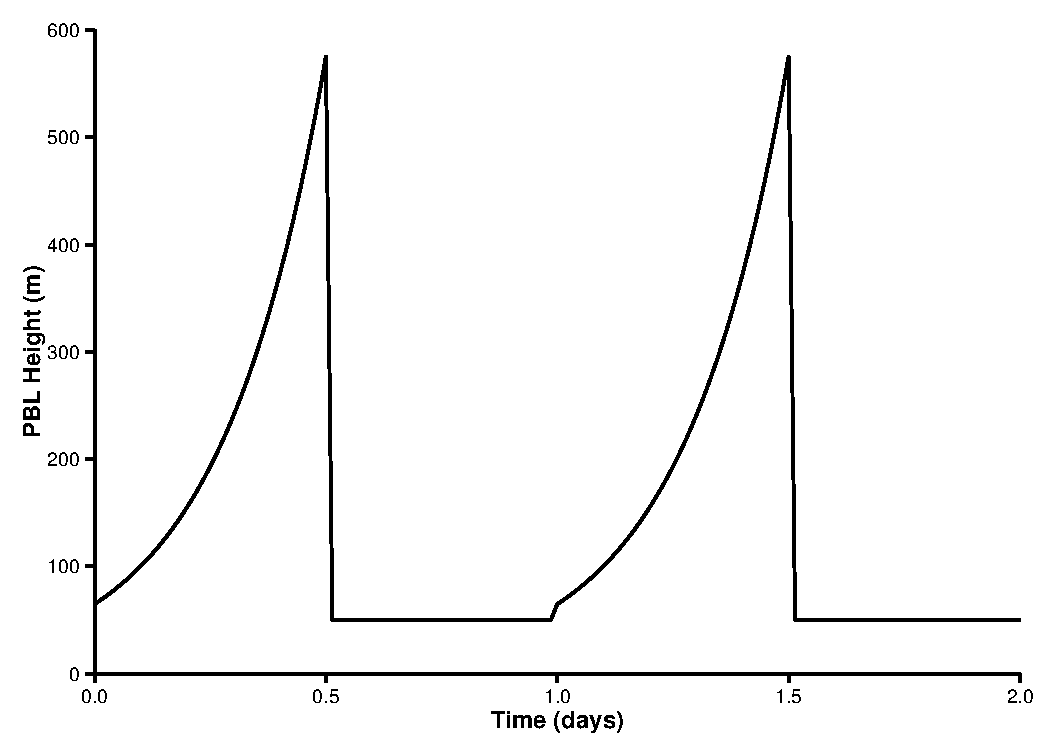
\includegraphics[width=\textwidth]{img/PBL_time_series}
\end{figure}
